\subsection{向量丛的定义}

7.1.1. 一个向量丛图 \(t = (U, \varphi, F)\) 是 M 的一个三元组，其中 U 是 B 的开子集，F 是巴拿赫空间，而 \(\varphi\) 是从 \(\pi^{-1}(U)\) 到 \(U \times F\) 的双射，满足 \(\pi(\varphi^{-1}(b, h)) = b\)，对所有 \(b \in B\) 和所有 \(h \in F\) 均成立。我们称 U 为向量丛图 \(t\) 的定义域，并称 \(t\) 是 M 在 \(b \in B\) 处的向量丛图，当 \(b \in U\) 时。对每个 \(b \in U\)，记 \(t_b\) 为从 F 到 \(M_b\) 的双射，其定义为 \(t_b(h) = \varphi^{-1}(b, h)\)，其中 \(h \in F\)。

7.1.2. 设 \(t = (\mathrm{U}, \varphi, \mathrm{F})\) 和 \(t' = (\mathrm{U}', \varphi', \mathrm{F}')\) 是 \(\mathbf{M}\) 的两个向量丛图。它们称为 \(\mathbf{C}'\)-相容（或简称相容），当且仅当存在一个映射 \(\lambda\)，其类为 \(\mathbf{C}'\)，从流形 \(\mathrm{U} \cap \mathrm{U}'\) 到巴拿赫空间 \(\mathcal{L}(\mathrm{F}; \mathrm{F}')\)，使得：

\[
t _ {b} = t _ {b} ^ {\prime} \circ \lambda (b) \quad \text { for all } b \in \mathbf {U} \cap \mathbf {U} ^ {\prime}.
\]

7.1.3. M 的一组向量丛图称为 M 的 C'-向量丛图册（或简称向量丛图册），如果它由两两 C'-相容且定义域的并为 B 的向量丛图组成。M 的两个向量丛图册 A 和 B 称为 C'-等价（或等价），如果 A ∪ B 仍是 M 的向量丛图册。这个关系是一个等价关系。

7.1.4. M 上的类为 \(C^{r}\) 的向量丛结构（基底 B）是一个等价向量丛图册类的数据（《集合论》，第 II 章，第 6 节，第 9 号）。属于这个类中某个向量丛图册的向量丛图称为向量丛 M 的向量丛图。

设 M 是以 B 为基底的向量丛。对每个 \(b \in B\)，纤维 \(M_{b}\) 上存在唯一一个巴拿赫空间结构，使得对于向量丛 M 在 b 处的每个向量丛图 \(t = (\mathbf{U}, \varphi, \mathbf{F})\)，映射 \(t_{b}\) 都是从 F 到 \(M_{b}\) 的同构。

设 \(c = (\mathbf{U}, \psi, \mathbf{E})\) 是流形 \(\mathbf{B}\) 的一个图，\(t = (\mathbf{U}, \varphi, \mathbf{F})\) 是向量丛 \(\mathbf{M}\) 的一个向量丛图，二者有相同的定义域 \(\mathbf{U}\)。对 \(x \in \pi^{-1}(\mathbf{U})\)，置：

\[
\alpha (x) = (\psi (\pi (x)), t _ {\pi (x)} ^ {- 1} (x)).
\]

于是，三元组 \((\pi^{-1}(\mathbf{U}), \alpha, \mathbf{E} \times \mathbf{F})\) 是集合 M 的一个图。M 上存在唯一一个类为 \(C^{r}\) 的流形结构（称为 M 的底层结构），使得如此得到的所有图都是流形 M 的图。于是三元组 \((\mathbf{M}, \mathbf{B}, \pi)\) 是一个纤维化（6.1.1）。

7.1.5. 设 F 是一个巴拿赫空间。置 \(M = B \times F\)，其中映射取为第一投影。M 上存在唯一一个向量丛结构（以 B 为基底），使得 \((\mathbf{B}, \mathbf{Id}_{\mathbf{M}}, \mathbf{F})\) 是一个向量丛图。我们称赋予此结构的 \(B \times F\) 为以 B 为基底、纤维为 F 的平凡向量丛，有时记为 \(F_{B}\)。\(F_{B}\) 的流形结构是乘积流形结构，并且对于每个 \(b \in B\)，映射 \(h \mapsto (b, h)\) 是从 F 到 \(F_{B}\) 的纤维的巴拿赫空间同构，该纤维位于点 \(b \in B\) 处。纤维退化为 0 的平凡向量丛通常记为 0。

7.1.6. 设 M 是以 B 为基底的向量丛。对于 \(b \in B\)，将（有限或 \(+\infty\) 的）巴拿赫空间 \(M_{b}\) 的维数称为 M 在 b 处的秩，记为 \(\operatorname{rg}_{b}(\mathbf{M})\)。有 \(\dim_{x}\mathbf{M} = \dim_{b}\mathbf{B} + \operatorname{rg}_{b}\mathbf{M}\)，其中 \(b = \pi(x)\)。函数 \(b \mapsto \operatorname{rg}_{b}\mathbf{M}\) 局部常值。若满足 \(\operatorname{rg}_{b}\mathbf{M} < +\infty\) 对所有 \(b \in B\)，则称 M 是有限秩的。

\subsection{向量丛的态射}

7.2.1. 设 B 和 B' 是两个流形，f 是从 B 到 B' 的态射。设 M 是以 B 为基底的向量丛，M' 是以 B' 为基底的向量丛。如果满足以下条件，则称从 M 到 M' 的映射 g 为向量丛的 f-态射：

对于每个点 \(b_0 \in \mathbf{B}\)，存在一个向量丛图 \(t = (\mathrm{U}, \varphi, \mathrm{F})\)，它属于 \(\mathbf{M}\)，在点 \(b_0\) 处；存在一个向量丛图 \(t' = (\mathrm{U}', \varphi', \mathrm{F}')\)，它属于 \(\mathbf{M}'\)，在点 \(f(b_0)\) 处；以及一个映射 \(\lambda\)，其类为 \(\mathbf{C}'\)，从 \(\mathbf{U}\) 到 \(\mathcal{L}(\mathbf{F}; \mathbf{F}')\)，使得 \(f(\mathbf{U}) \subset \mathbf{U}'\)，并且 \(g_b \circ t_b = t_{f(b)}' \circ \lambda(b)\) 对所有 \(b \in \mathbf{U}\) 都成立，其中 \(g_b\) 是 \(g\) 在 \(\mathbf{M}_b\) 上的限制。

在这些假设下，\(g\) 是流形的态射，并且对每个 \(b \in B\)，\(g\) 诱导出从 \(M_b\) 到 \(M_{f(b)}'\) 的连续线性映射。称（有限或 \(+\infty\) 的）线性映射 \(g_b\) 的秩为 \(g\) 在 \(b \in B\) 处的向量秩，记为 \(\text{rg}_b(g)\)。

反之，若 \(r \geqslant \infty\)，或 \(M\) 是有限秩的，则对于给定的 \(f\)，从纤维化 \((M, B, \pi)\) 到 \((M', B', \pi')\) 的态射，若在每个纤维 \(M_b\) 上诱导出从 \(M_b\) 到 \(M_{f(b)}'\) 的线性映射（对每个 \(b \in B\)），则是向量丛的 \(f\)-态射。

7.2.2. 此外，设 \(f'\) 是从 \(B'\) 到流形 \(B''\) 的态射。如果 \(g\) 是一个 \(f\)-态射，从 \(M\) 到 \(M'\)，且 \(g'\) 是一个 \(f'\)-态射，从 \(M'\) 到向量丛 \(M''\)，其基底为 \(B''\)，则映射 \(g' \circ g\) 是一个 \((f' \circ f)\)-态射，从 \(M\) 到 \(M''\)。有 \((g' \circ g)_b = g_{f(b)}' \circ g_b\)，其中 \(b\) 遍历 \(B\)。

7.2.3. 设 M 和 M' 是以同一个 B 为基底的两个向量丛。B-态射，或简称从 M 到 M' 的态射，是任意一个 \(\mathrm{Id}_{\mathbf{B}}\)-态射。两个态射的复合是一个态射。

设 \(g\) 是从 \(M\) 到 \(M'\) 的向量丛态射；若 \(g\) 是双射，则它是从流形 \(M\) 到流形 \(M'\) 的同构，逆映射 \(g^{-1}\) 是从 \(M'\) 到 \(M\) 的向量丛态射，并且 \((g^{-1})_b = g_b^{-1}\) 对所有 \(b\) 属于 \(B\) 都成立。此时映射 \(g\) 称为向量丛同构。

7.2.4. 设 \(f\) 是从流形 \(\mathbf{B}'\) 到 \(\mathbf{B}\) 的态射，并设 \(\mathbf{M}\) 是以 \(\mathbf{B}\) 为基底的向量丛。置 \(\mathbf{M}' = \mathbf{B}' \times_{\mathbf{B}} \mathbf{M}\)，并记为 \(\pi'\)（分别记为 \(g\)），它们是投影在 \(\mathbf{M}'\) 上的限制；这里的投影从 \(\mathbf{B}' \times \mathbf{M}\) 到 \(\mathbf{B}'\)（分别到 \(\mathbf{M}\)）。在 \(\mathbf{M}'\) 上存在一个以 \(\mathbf{B}'\) 为基底（相对于 \(\pi'\)）的向量丛结构，并且只有一个这样的结构使 \(g\) 成为 \(f\)-态射。称 \(\mathbf{M}'\) 为以 \(\mathbf{B}'\) 为基底的 \(\mathbf{M}\) 由 \(f\) 逆向拉回的向量丛，记为 \(f^* \mathbf{M}\)；这个 \(f\)-态射 \(g\) 称为典范 \(f\)-态射，从 \(f^* \mathbf{M}\) 到 \(\mathbf{M}\)。

\(f^{*}\mathbf{M}\) 的流形结构就是流形 \(\mathbf{B}'\) 与 \(\mathbf{M}\) 在 \(\mathbf{B}\) 上的纤维积的流形结构（5.11.2）；对每个 \(b\in\mathbf{B}'\)，映射 \(x\mapsto(b,x)\) 是从 \(\mathbf{M}_{f(b)}\) 到 \((f^{*}\mathbf{M})_{b}\) 的巴拿赫空间同构。

向量丛逆像的构造具有传递性。

设 N' 是以 B' 为基底的向量丛，h 是从 N' 到 M 的 f-态射。存在唯一一个 B'-态射 \(\tilde{h}\)，它从 N' 到 \(f^{*}M\)，使得 \(h = g \circ \tilde{h}\)。

设 N 是以 B 为基底的向量丛，v 是从 N 到 M 的 B-态射。存在唯一一个记为 \(f^{*}v\) 的 B'-态射，从 \(f^{*}N\) 到 \(f^{*}M\)，使得下图

\pandocbounded{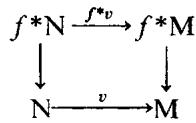
\includegraphics[keepaspectratio]{images/part001_e53c46a7.jpg}}

交换。

7.2.5. 设 B' 是 B 的子流形，i 是从 B' 到 B 的典范嵌入。若 M 是以 B 为基底的向量丛，则 \(i^*M\) 称为 M 在 B' 上诱导的向量丛，记为 \(M|_{B'}\)。若 \(t = (\mathrm{U}, \varphi, \mathrm{F})\) 是 M 的一个向量丛图，则 \((\mathrm{U} \cap \mathrm{B}', \varphi | \pi^{-1}(\mathrm{U} \cap \mathrm{B}'), \mathrm{F})\) 是 \(M|_{B'}\) 的一个向量丛图。从 \(M|_{B'}\) 到 M 的典范 f-态射是从 \(M|_{B'}\) 到 M 的子流形 \(\pi^{-1}(\mathrm{B}')\) 的一个流形同构。

7.2.6. 设 \(f\) 是从流形 B' 到 B 的态射，M（分别 M'）是以 B（分别 B'）为基底的向量丛。从 M 到 M' 的 \(f\)-余态射定义为从 \(f^{*}M\) 到 M' 的 B'-态射。当 B = B' 且 \(f = \mathrm{Id}_{\mathbf{B}}\) 时，从 M 到 M' 的 f-余态射的数据等价于从 M 到 M' 的 B-态射的数据。

设 \(g\) 是一个 \(f\)-余态射，从 \(\mathbf{M}\) 到 \(\mathbf{M}'\)。对每个 \(b \in \mathbf{B}'\)，映射 \(g_b: x \mapsto g(b, x)\) 从 \(\mathbf{M}_{f(b)}\) 到 \(\mathbf{M}_b'\)，是连续线性映射。

此外，设 \(f'\) 是从流形 \(B''\) 到 \(B'\) 的态射，且 \(h\) 是一个 \(f'\)-余态射，从 \(M'\) 到向量丛 \(M''\)，其基底为 \(B''\)。于是，映射 \(h \circ f'^{*}g\)，其定义域为 \(f'^{*}(f^{*}M) = (f \circ f')^{*}M\)，值域为 \(M''\)，是 \((f \circ f')\)-余态射，从 \(M\) 到 \(M''\)，记为 \(h \circ g\)。对于 \(b \in B''\)，有

\[
(h \circ g) _ {b} = h _ {b} \circ g _ {f ^ {\prime} (b)}.
\]

\subsection{多线性态射}

7.3.1. 设 \(M_{1},\ldots,M_{d}\) 和 N 是以 B 为基底的向量丛，u 是从集合 \(M_{1}\times_{B}\ldots\times_{B}M_{d}\) 到 N 的映射。如果满足以下条件，则称 u 为多线性态射（或 d-线性态射）：

对于每个 \(b_0 \in \mathbf{B}\)，存在一个开邻域 \(\mathbf{U}\)，包含 \(b_0\) 且位于 \(\mathbf{B}\) 中，存在向量丛图 \(t^j = (\mathbf{U}, \varphi^j, \mathbf{F}^j)\)，它们属于 \(\mathbf{M}_j\)（\(1 \leqslant j \leqslant d\)），以及向量丛图 \(t = (\mathbf{U}, \varphi, \mathbf{F})\)，它属于 \(\mathbf{N}\)，还有映射 \(\lambda\)，其类为 \(\mathbf{C}^r\)，从 \(\mathbf{U}\) 到巴拿赫空间 \(\mathcal{L}(\mathbf{F}^1, \ldots, \mathbf{F}^d; \mathbf{F})\)，该空间由从 \(\mathbf{F}^1 \times \cdots \times \mathbf{F}^d\) 到 \(\mathbf{F}\) 的连续 d-线性映射组成，使得：

\[
(t _ {b} \circ \lambda (b)) (x _ {1}, \dots , x _ {d}) = u (t _ {b} ^ {1} (x _ {1}), \dots , t _ {b} ^ {d} (x _ {d}))
\]

对所有 \(b \in \mathbf{U}\) 和所有 \(x_{j} \in \mathbf{F}^{j}\) 都成立。

每个多线性态射 \(u\) 都是从纤维积 \(\mathbf{M}_{1} \times_{\mathbf{B}} \cdots \times_{\mathbf{B}} \mathbf{M}_{d}\) 到 \(\mathbf{N}\) 的流形态射，并且对每个 \(b \in \mathbf{B}\) 诱导出一个连续 \(d\)-线性映射 \(u_b\)，从 \((\mathbf{M}_{1})_{b} \times \cdots \times (\mathbf{M}_{d})_{b}\) 到 \(\mathbf{N}_{b}\)。

若 \(f\) 是从 B 到流形 \(\mathbf{B}'\) 的态射，则从 \(\mathbf{M}_1 \times_{\mathbf{B}} \cdots \times_{\mathbf{B}} \mathbf{M}_d\) 到向量丛 \(\mathbf{M}'\)（其基底为 \(\mathbf{B}'\)）的多线性态射，按定义是从 \(\mathbf{M}_1 \times_{\mathbf{B}} \cdots \times_{\mathbf{B}} \mathbf{M}_d\) 到 \(f^*\mathbf{M}'\) 的多线性态射与由 \(f\) 给出的从 \(f^*\mathbf{M}'\) 到 \(\mathbf{M}'\) 的典范态射的复合。

双线性态射也称为配对。当 \(d=1\) 时，线性态射就是 7.2.1 意义下的态射。当 \(d=0\) 时，0-线性态射与 N 的一个截面（7.4）等同。

7.3.2. 以 B 为基底的代数丛是以 B 为基底、配备了从 \(A \times_{B} A\) 到 A 的配对的向量丛 A。于是每个纤维 \(A_{b}\) 都带有一个 K-代数结构。若对每个 \(b \in B\)，代数 \(A_{b}\) 有单位元，记为 \(e_{b}\)，则映射 \(b \mapsto e_{b}\) 是 A 的一个截面（参见 7.4）。如果对 B 中每个点 \(b_{0}\)，都存在一个向量丛图 \(t = (\mathrm{U}, \varphi, \mathrm{E})\)，它属于 A 并在点 \(b_{0}\) 处，以及 E 上的 K-代数结构，使得 \(t_{b}\) 是从 E 到 \(A_{b}\) 的代数同构，对所有 \(b \in U\) 均如此，则称代数丛 A 是局部平凡的。

7.3.3. 设 A 是以 B 为基底的带单位元的结合代数丛。以 B 为基底的 A-模丛定义为以 B 为基底的向量丛 M，配备一个配对 \(m: A \times_{B} M \to M\)，使得映射 \(m_{b}: A_{b} \times M_{b} \to M_{b}\) 对每个 \(b \in B\) 定义出 \(A_{b}\) 在纤维 \(M_{b}\) 上的模结构。

设 M 和 M′ 是两个 A-模向量丛。从 M 到 M′ 的 A-同态定义为以 B 为基底的向量丛态射 \(g: M \rightarrow M'\)，它对 B 中每个 b 都诱导出一个 \(A_b\)-线性映射，从 \(M_b\) 到 \(M_b'\)。

设 A 是局部平凡的。若对 B 中每个点 \(b_0\)，都存在一个向量丛图 \(t = (U, \varphi, E)\)，它是如 7.3.2 中所述的 A 在 \(b_0\) 处的图；另有一个向量丛图 \(t' = (U, \varphi', L)\)，它是 M 在 \(b_0\) 处的图；以及 L 上的 E-模结构，使得对每个 \(b \in U\)，\(t_b'\) 是 \(t_b\)-同构，将 \(A_b\)-模 \(M_b\) 映到 E-模 L，则称 A-模丛 M 是局部平凡的。

7.3.4. 设 A 是 K 上的巴拿赫代数（例如，带有有限维 K-代数结构的域）。平凡丛 \(A_{B}\) 于是是一个局部平凡代数丛。A-模 \(A_{B}\) 中的局部平凡丛 M 也称为 A 上的向量丛（以 B 为基底）。于是纤维 \(M_{b}\) 是拓扑 A-模。从 M 到另一个 A 上的向量丛的 f-态射 u 称为 A-线性的，如果映射 \(u_{b}\) 对所有 \(b \in B\) 都是 A-线性的。

\subsection{截面}

7.4.1. 设 M 是以 B 为基底的向量丛。对 B 的每个开集 U，记 \(\mathcal{S}_{\mathbf{M}}^{r}(\mathbf{U})\) 为 M 在 U 上的类为 \(C^r\) 的截面集，即从 U 到 M 的态射 \(s\)，其类为 \(C^r\)，满足 \(s(b) \in M_b\) 对所有 \(b \in \mathbf{U}\) 都成立。根据以下规则，这个集合带有关于态射函数环 \(\mathcal{C}^r(\mathbf{U})\) 的模结构：

\begin{enumerate}
\def\labelenumi{(\arabic{enumi})}
\tightlist
\item
\end{enumerate}

\[
(s + s ^ {\prime}) (b) = s (b) + s ^ {\prime} (b)\tag{2}
\]

\[
(\varphi . s) (b) = \varphi (b). s (b)
\]

其中 \(s, s'\) 属于 \(\mathcal{S}_{\mathrm{M}}^{r}(\mathrm{U})\)，\(\varphi\) 属于 \(\mathcal{C}^{r}(\mathrm{U})\)。当开集 U 变化时，得到一个从 B 到 M 的映射层 \(\mathcal{S}_{\mathrm{M}}^{r}\)（参见第 5.4.1 号），称为 M 的截面层。

7.4.2. 设 \(M_{1},\ldots,M_{d}\) 和 N 是以 B 为基底的向量丛，u 是从 \(M_{1}\times_{B}\ldots\times_{B}M_{d}\) 到 N 的多线性态射。对 \(1\leqslant j\leqslant d\)，给定一个截面 \(s_{j}\)，它是 \(M_{j}\) 在 B 的一个开集 U 上的截面；按下式在 U 上定义 N 的截面 \(u(s_{1},\ldots,s_{d})\)：

\[
u (s _ {1}, \dots , s _ {d}) (b) = u _ {b} (s _ {1} (b), \dots , s _ {d} (b)) \quad \text {   for   } b \in \mathrm{U}.
\]

映射 \((s_1, \ldots, s_d) \mapsto u(s_1, \ldots, s_d)\) 是 \(\mathcal{C}^r(\mathrm{U})\)-多线性的，有时记为 \(\mathcal{S}(u)\)。

7.4.3. 设 \(f\) 是从流形 \(\mathbf{B}'\) 到 \(\mathbf{B}\) 的态射，\(\mathbf{M}\) 是以 \(\mathbf{B}\) 为基底的向量丛。对每个开集 \(\mathbf{U}\)，它属于 \(\mathbf{B}\)，以及每个 \(s \in \mathcal{S}_{\mathbf{M}}^{r}(\mathbf{U})\)，映射 \(x \mapsto (x, s(f(x)))\) 是类为 \(\mathbf{C}^r\) 的 \(f^{*}\mathbf{M}\) 在开子集 \(f^{-1}(\mathbf{U})\) 上的截面，记为 \(f^{*}s\)，称为 \(s\) 关于 \(f\) 的逆像。映射 \(s \mapsto f^{*}s\) 从 \(\mathcal{S}_{\mathbf{M}}^{r}(\mathbf{U})\) 到 \(\mathcal{S}_{f^{*}\mathbf{M}}^{r}(f^{-1}(\mathbf{U}))\) 关于同态 \(g \mapsto g \circ (f|f^{-1}(\mathbf{U}))\)（它从 \(\mathcal{C}^{r}(\mathbf{U})\) 到 \(\mathcal{C}^{r}(f^{-1}(\mathbf{U}))\)）是半线性的。

此外，若 N 是以 B' 为基底的向量丛，g 是从 M 到 N 的 f-余态射，有时将记为 \(\mathcal{S}(g)\) 的映射 \(s \mapsto g \circ f^{*}s\) 从 \(\mathcal{S}_{\mathbf{M}}^{\mathbf{r}}(\mathbf{U})\) 到 \(\mathcal{S}_{\mathbf{N}}^{\mathbf{r}}(f^{-1}(\mathbf{U}))\)。

7.4.4. 设 M 是以 B 为基底的有限秩向量丛。M 在 B 的一个开集 U 上的标架定义为 M 在 U 上的截面组成的有限序列 \((s_{1},\ldots,s_{n})\)，使得 \((s_{1}(b),\ldots,s_{n}(b))\) 是向量空间 \(M_{b}\) 的一个基，对所有 \(b\in U\) 均如此。于是序列 \((s_{1},\ldots,s_{n})\) 是 \(\mathcal{C}^{r}(\mathrm{U})\)-模 \(\mathcal{S}_{\mathbf{M}}^{r}(\mathrm{U})\) 的一个基。若 f 是从流形 \(B'\) 到 B 的态射，则截面 \(f^{*}s_{j}\) 构成 \(f^{*}\mathbf{M}\) 在 \(f^{-1}(\mathbf{U})\) 上的一个标架。

7.4.5. 设 L 是一个赋有有限维 K-代数结构的域，(M, B, π) 是一个纤维化。假定每个纤维 \(M_{b}\) 上都给定了有限维的 L-向量空间结构。M 上至多存在一个以 B 为基底的向量丛结构，它与映射 π、M 的流形结构以及各纤维上的 L-向量空间结构相容（7.3.4）。这种结构存在的充要条件是满足以下条件：

（FV）对每个 \(b_0 \in \mathbf{B}\)，存在一个开邻域 \(\mathbf{U}\)，其中包含 \(b_0\) 且位于 \(\mathbf{B}\) 中，以及一个流形同构 \(\varphi\)，它从 \(\pi^{-1}(\mathbf{U})\) 到乘积 \(\mathbf{U} \times \mathbf{F}\)，它是 \(\mathbf{U}\) 与 \(\mathbf{F}\) 的乘积，其中后者是有限维的 \(\mathbf{L}\)-向量空间，使得对每个 \(b \in \mathbf{U}\)，双射 \(\varphi_b\) 从 \(\mathbf{M}_b\) 到 \(\mathbf{F}\) 由 \(\varphi\) 诱导，并且是 \(\mathbf{L}\) 上的向量空间同构。

于是，满足（FV）的三元组（U，\(\varphi\)，F）就是向量丛 M 的向量丛图。

条件（FV）等价于：

（FV'）对每个 \(b_0 \in \mathbf{B}\)，存在一个整数 \(n\) 以及 \(n\) 个截面 \(s_1, \ldots, s_n\)，它们是 \(\mathbf{M}\) 在开邻域 \(\mathbf{U}\) 上的截面，而该邻域包含 \(b_0\)，使得映射

\[
(b, a _ {1}, \dots , a _ {n}) \mapsto a _ {1} s _ {1} (b) + \dots + a _ {n} s _ {n} (b)
\]

是从流形 \(\mathbf{U} \times \mathbf{L}^{n}\) 到流形 \(\pi^{-1}(\mathbf{U})\) 的同构。

7.4.6. 设 \(M_{1},\ldots,M_{d}\) 和 N 是以 B 为基底的向量丛，其中 \(M_{j}\) 为有限秩。假定对 B 的每个开集 U，都给定了一个 \(\mathcal{C}^{r}(\mathrm{U})\)-多线性映射 \(\varphi_{\mathrm{U}}\)，从 \(\mathcal{S}_{\mathrm{M}_{1}}^{\mathrm{r}}(\mathrm{U})\times\cdots\times\mathcal{S}_{\mathrm{M}_{d}}^{\mathrm{r}}(\mathrm{U})\) 到 \(\mathcal{S}_{\mathrm{N}}^{\mathrm{r}}(\mathrm{U})\)，使得当 \(V \subset U\) 时有：

\[
\varphi_ {\mathrm{U}} (s _ {1}, \dots , s _ {d}) | \mathrm{V} = \varphi_ {\mathrm{V}} (s _ {1} | \mathrm{V}, \dots , s _ {d} | \mathrm{V}).
\]

于是存在一个多线性态射 \(u\)，从 \(\mathbf{M}_1 \times_{\mathbf{B}} \ldots \times_{\mathbf{B}} \mathbf{M}_d\) 到 \(\mathbf{N}\)，使得 \(\varphi_{\mathbf{U}}(s_1, \ldots, s_d) = u(s_1, \ldots, s_d)\) 对任意截面 \(s_j\)，属于 \(\mathbf{M}_j\) 在开集 \(\mathbf{U}\)（属于 \(\mathbf{B}\)）上的截面，均成立。

7.4.7. 设 \(f\) 是从流形 \(\mathbf{B}'\) 到 \(\mathbf{B}\) 的态射，且 \(\mathbf{M}\)（分别 \(\mathbf{M}'\)）是以 \(\mathbf{B}\)（分别 \(\mathbf{B}'\)）为基底的有限秩向量丛。假定对每个开集 \(\mathbf{U}\)，它属于 \(\mathbf{B}\)，给定一个连续的 \(\mathcal{C}^{r}(\mathbf{U})\)-半线性映射 \(\varphi_{\mathbf{U}}\)，从 \(\mathcal{S}_{\mathbf{M}}^{r}(\mathbf{U})\) 到 \(\mathcal{S}_{\mathbf{M}'}^{r}(f^{-1}(\mathbf{U}))\)，使得

\[
\varphi_ {\mathbf {U}} (s) | f ^ {- 1} (\mathbf {V}) = \varphi_ {\mathbf {V}} (s | \mathbf {V})
\]

对每个开集 \(V \subset U\) 都有。于是存在唯一一个从 M 到 \(M'\) 的 f-余态射 g，使得 \(\varphi_{\mathrm{U}}(s) = \mathcal{S}(g)(s)\) 对所有 \(s \in \mathcal{S}_{\mathrm{M}}^{r}(\mathrm{U})\) 都成立。

*7.4.8. 设 \(\mathcal{F}\) 是关于环层 \(\mathcal{C}_{\mathrm{B}}^{r}\) 的模层。我们称 \(\mathcal{F}\) 是局部自由的：对每个 \(b \in \mathrm{B}\)，存在一个开邻域 U，含有 \(b\)，以及一个整数 \(n\)，使得 \(\mathcal{F}|\mathrm{U}\) 与一个 \(\mathcal{C}_{\mathrm{U}}^{r}\)-模层 \((\mathcal{C}_{\mathrm{U}}^{r})^{n}\) 同构。

若 M 是以 B 为基底的有限秩向量丛，则层 \(\mathcal{S}_{\mathrm{M}}^{r}\) 是局部自由的。反之，对 B 上每个局部自由层 \(\mathcal{F}\)，存在一个向量丛 M 以及从 \(\mathcal{S}_{\mathrm{M}}^{r}\) 到 \(\mathcal{F}\) 的层同构。若 M' 是另一个以 B 为基底的有限秩向量丛，则映射 \(g \mapsto \mathcal{S}(g)\) 是从 M 到 M' 的 B-态射集到从 \(\mathcal{C}^{r}\)-模层态射 \(\mathcal{S}_{\mathrm{M}}^{r}\) 到 \(\mathcal{S}_{\mathrm{M}'}^{r}\) 的集合的双射。

\subsection{子向量丛、商向量丛、正合序列}

本号中，向量丛均指以 B 为基底的向量丛，向量丛态射均指 \(\mathrm{Id}_{\mathbf{B}}\)-态射。

7.5.1. 设 M 是一个向量丛。如果对每个点 \(b \in B\)，都存在 M 在 b 处的向量丛图 \(t = (\mathbf{U}, \varphi, \mathbf{E})\) 以及 E 的一个具有拓扑补空间的闭向量子空间 F，使得

\[
\varphi (\pi^ {- 1} (\mathrm{U}) \cap \mathrm{M} ^ {\prime}) = \mathrm{U} \times \mathrm{F}.
\]

在这些条件下，M′ 上存在唯一一个向量丛结构，使得从 M′ 到 M 的典范嵌入是一个态射。对每个 \(b \in B\)，M' 的纤维 \(M_{b}'\) 是闭向量子空间 \(M' \cap M_{b}\)，并且该空间包含于 \(M_{b}\)；M' 是 M 的闭子流形，并且 M' 的向量丛结构的底层流形结构与由 M 的流形结构诱导的结构一致。

7.5.2. 设 M' 是 M 的一个子向量丛。用 R 表示 M 的点 x、y 之间的如下关系：

存在 \(b\) 属于 \(B\)，使得 \(x \in M_b, y \in M_b\) 且 \(x - y \in M_b'\)。于是 \(R\) 是 \(M\) 上的正则等价关系（参见第 5.9.7 号）。集合 \(M/R\) 上存在唯一一个向量丛结构，使得从 \(M\) 到 \(M/R\) 的典范映射是一个态射。将其记为 \(M/M'\)，并称 \(M\) 对 \(M'\) 的商为如此定义的向量丛；对于 \(b\) 属于 \(B\) 的每个点，丛 \((M/M')_b\) 是商拓扑向量空间 \(M_b/M_b'\)，而 \(M/M'\) 上的流形结构是 \(M\) 上流形结构的商结构。

7.5.3. 保留 7.5.2 的假设。对于 B 的每个点 \(b_0\)，可以找到一个开邻域 U，其中包含 \(b_0\)；一个巴拿赫空间 F，它是两个闭子空间 \(F'\) 和 \(F''\) 的直和；以及一个向量丛同构 \(\iota\)，从 \(\mathbf{F}_{\mathbf{U}}\) 到 \(\mathbf{M}|\mathbf{U}\)，满足以下性质：

\begin{enumerate}
\def\labelenumi{(\roman{enumi})}
\item
  \(\iota'\) 是 \(\iota\) 在 \(\mathbf{U} \times \mathbf{F}'\) 上的限制，并且是从 \(\mathbf{F}_{\mathbf{U}}'\) 到 \(\mathbf{M}'|\mathbf{U}\) 的同构。
\item
  若 \(\rho\) 是从 M 到 \(\mathbf{M}'' = \mathbf{M} / \mathbf{M}'\) 的典范映射，且 \(\iota''\) 是 \(\iota\) 在 \(\mathbf{U} \times \mathbf{F}''\) 上的限制，则映射 \(\rho \circ \iota''\) 是从 \(\mathbf{F}_{\mathbf{U}}''\) 到 \(\mathbf{M}''|\mathbf{U}\) 的同构。
\end{enumerate}

7.5.4. 若向量丛态射 \(g: \mathbf{L} \to \mathbf{M}\) 的像包含于 \(\mathbf{M}'\)，则它是从 \(\mathbf{L}\) 到 \(\mathbf{M}'\) 的向量丛态射。

现在设 \(h: \mathbf{M} \to \mathbf{N}\) 是一个向量丛态射，并假定对 B 中的每个 \(b\)，\(h_b\) 在 \(\mathbf{M}_b'\) 上的限制为零。若 \(\rho\) 是从 M 到 \(\mathbf{M}/\mathbf{M}'\) 的典范态射，则存在唯一一个态射 \(\bar{h}\)，其从 \(\mathbf{M}/\mathbf{M}'\) 到 N，且满足 \(h = \bar{h} \circ \rho\)。

7.5.5. 设 P、Q 是两个向量丛，g 是从 P 到 Q 的态射；对 B 中的每个点 b，分别以 \(N_{b}\) 和 \(I_{b}\) 表示线性映射 \(g_{b}:P_{b}\to Q_{b}\) 的核和像。置 \(N=\bigcup_{b\in B}N_{b}\)，以及

\(I = \bigcup_{b \in B} I_b\)。称态射 \(g\) 是局部直的，当且仅当 \(N\) 是 P 的子向量丛且 I 是 Q 的子向量丛。于是态射 g 通过取商定义了从 P/N 到 I 的同构。称 N 为 g 的核，记为 Ker g。同样，子丛 I 称为 g 的像，记为 Im g。

若 \(r \geqslant \infty\)，则态射 \(g\) 局部直当且仅当 \(g\) 是子浸入。若 P 是有限秩的，则态射 \(g\) 局部直当且仅当 \(g\) 的向量秩局部常值，或者等价地，当且仅当 \(g\) 是子浸入。

7.5.6. 设 \(\mathbf{M} \xrightarrow{f} \mathbf{M}' \xrightarrow{g} \mathbf{M}''\) 是两个向量丛态射。称序列 \((f, g)\) 是局部直正合的，当且仅当 \(f\) 和 \(g\) 都局部直且 \(\operatorname{Im} f = \operatorname{Ker} g\)。若 \(g \circ f = 0\)，令 \(\mathbf{D}\) 为满足以下条件的点 \(b \in \mathbf{B}\) 的集合：序列 \(\mathbf{M}_b \xrightarrow{f_b} \mathbf{M}_b' \xrightarrow{g_b} \mathbf{M}_b''\) 是直正合的（即 \(\operatorname{Ker} f_b\) 和 \(\operatorname{Im} g_b\) 有拓扑补空间，且 \(\operatorname{Im} f_b = \operatorname{Ker} g_b\)）。则 D 是开集，并且序列 \(\mathbf{M}|\mathbf{D} \xrightarrow{f} \mathbf{M}'|\mathbf{D} \xrightarrow{g} \mathbf{M}''|\mathbf{D}\) 是局部直正合的。

任意长度的局部直正合序列也以同样方式定义。语言上滥用时，有时用“直正合序列”代替“局部直正合序列”。

7.5.7. 设 \(0 \to \mathbf{M} \xrightarrow{f} \mathbf{M}' \xrightarrow{g} \mathbf{M}'' \to 0\) 是一个向量丛态射序列。这个序列局部直正合的充要条件是：\(f\) 是从 \(\mathbf{M}\) 到子向量丛 \(f(\mathbf{M})\) 的同构，该子丛属于 \(\mathbf{M}'\)，并且 \(g\) 通过取商定义了从商向量丛 \(\mathbf{M}'/f(\mathbf{M})\) 到 \(\mathbf{M}''\) 的同构。

\subsection{向量函子}

本号以及其后的三个 7.7 至 7.9 号中，字母 I 表示一个有限集，它是两个不交子集 \(I_+\) 和 \(I_-\) 的并。我们用 \(\mathcal{V} = (\mathrm{V}_{i})_{i\in I}\)（\(\mathcal{V}'\)、\(\mathcal{V}''\)、\ldots）也同样表示一个由 I 编号的巴拿赫空间族。我们用 \(\operatorname{Hom}(\mathcal{V},\mathcal{V}')\) 表示巴拿赫空间 \(\prod_{i\in I_+}\mathcal{L}(\mathrm{V}_i;\mathrm{V}_i')\times \prod_{i\in I_-}\mathcal{L}(\mathrm{V}_i';\mathrm{V}_i)\)。我们用 \(\mathbf{f} = (f_i)\) 表示 \(\operatorname{Hom}(\mathcal{V},\mathcal{V}')\) 的一个元素。将 \(\mathrm{Id}_{\mathcal{V}}\) 记为元素 \((\mathrm{Id}_{\mathrm{V}_i})_{i\in I}\)，它属于 \(\operatorname{Hom}(\mathcal{V},\mathcal{V})\)。对于 \(\mathbf{f}\in \operatorname{Hom}(\mathcal{V},\mathcal{V}')\) 和 \(\mathbf{f}'\in \operatorname{Hom}(\mathcal{V}',\mathcal{V}'')\)，用 \(\mathbf{f}'\circ \mathbf{f}\) 表示 \(\operatorname{Hom}(\mathcal{V},\mathcal{V}'')\) 中的元素，其分量由下式给出：

\[
\begin{array}{l l} (\mathbf {f} ^ {\prime} \circ \mathbf {f}) _ {i} = f _ {i} ^ {\prime} \circ f _ {i} & \text { if } \quad i \in \mathrm{I} _ {+} \\ (\mathbf {f} ^ {\prime} \circ \mathbf {f}) _ {i} = f _ {i} \circ f _ {i} ^ {\prime} & \text { if } \quad i \in \mathrm{I} _ {-}. \end{array}
\]

7.6.1. 类型为 I 且类为 \(\mathbf{C}^r\) 的向量函子（分别为有限维向量函子）是由如下数据组成的：对于每个由巴拿赫空间（分别为 K 上的有限维向量空间）组成的族 \(\mathcal{V} = (\mathrm{V}_i)_{i\in I}\)，给定一个巴拿赫空间 \(\tau(\mathcal{V})\)；对于每个 \(\mathbf{f}\in\mathrm{Hom}(\mathcal{V},\mathcal{V}')\)，给定一个元素 \(\tau(\mathbf{f})\in\mathcal{L}(\tau(\mathcal{V});\tau(\mathcal{V}'))\)；这些数据满足以下两个条件：

\begin{enumerate}
\def\labelenumi{(\alph{enumi})}
\item
  有 \(\tau (\mathrm{Id}_{\mathcal{V}}) = \mathrm{Id}_{\tau (\mathcal{V})}\)，且 \(\tau (\mathbf{f}'\circ \mathbf{f}) = \tau (\mathbf{f}')\circ \tau (\mathbf{f}).\)
\item
  映射 \(\tau : \operatorname{Hom}(\mathcal{V}, \mathcal{V}') \to \mathcal{L}(\tau(\mathcal{V}); \tau(\mathcal{V}'))\) 的类为 \(C'\)。
\end{enumerate}

7.6.2. 设 \(\mathcal{M} = (\mathbf{M}^i)_{i\in I}\) 是以 B 为基底的向量丛族。对 \(b\in \mathbf{B}\)，置 \(\mathcal{M}_b = (\mathbf{M}_b^i)_{i\in I}\)。设 \(\tau\) 是一个向量函子，并用 \(\tau (\mathcal{M})\) 表示所有 \(\tau(\mathcal{M}_{b})\) 的不交并，其中 \(b\in\mathbf{B}\)。

在 \(\tau(\mathcal{M})\) 上存在唯一一个向量丛结构（以 B 为基底，相对于映射 \(\pi\)，该映射从 \(\tau(\mathcal{M})\) 到 B），使得对每个 \(b\in\mathbf{B}\)，都有 \(\tau(\mathcal{M}_{b})=\pi^{-1}(b)\)，并且具有以下性质：

设 U 是 B 的一个开子集，并且对每个 i，设 \(t^{i} = (\mathrm{U}, \varphi_{i}, \mathrm{F}_{i})\) 是定义域为 U 的 \(M^{i}\) 的向量丛图；置 \(\mathcal{F} = (\mathrm{F}_{i})_{i \in I}\)，并令 \(\psi_{b}\) 为 \(\operatorname{Hom}(\mathcal{M}_{b}, \mathcal{F})\) 中的元素，满足 \((\psi_{b})_{i} = (t_{b}^{i})^{-1}\) 对 \(i \in I_{+}\) 成立，且 \((\psi_{b})_{i} = t_{b}^{i}\) 对 \(i \in I_{-}\) 成立；对 \(x \in \pi^{-1}(\mathrm{U})\)，置 \(\psi(x) = (\pi(x), \tau(\psi_{\pi(x)})(x))\)。则三元组 \((\mathrm{U}, \psi, \tau(\mathcal{F}))\) 是向量丛 \(\tau(\mathcal{M})\) 的一个向量丛图。

赋予这个结构后，\(\tau(\mathcal{M})\) 称为由向量丛族 \(\mathcal{M}\) 通过向量函子 \(\tau\) 导出的向量丛。

7.6.3. 设 \(f\) 是从 \(\mathbf{B}\) 到流形 \(\mathbf{B}'\) 的态射。设 \(\mathcal{M} = (\mathbf{M}^i)\)（分别 \(\mathcal{M}' = (\mathbf{M}'^i)\)）是由 \(\mathbf{I}\) 编号的、以 \(\mathbf{B}\)（分别 \(\mathbf{B}'\)）为基底的向量丛族。对每个 \(i \in \mathbf{I}_+\)，设 \(g_i\) 是一个 \(f\)-态射，从 \(\mathbf{M}^i\) 到 \(\mathbf{M}'^i\)；对每个 \(i \in \mathbf{I}_-\)，设 \(g_i\) 是一个 \(f\)-余态射，从 \(\mathbf{M}'^i\) 到 \(\mathbf{M}^i\)。置 \(\mathbf{g} = (g_i)_{i \in I}\)，并对 \(b \in B\) 置 \(\mathbf{g}_b = ((g_i)_b)_{i \in I}\)（参见 7.2.1 和 7.2.6）。存在一个 \(f\)-态射，记为 \(\tau(\mathbf{g})\)，从 \(\tau(\mathcal{M})\) 到 \(\tau(\mathcal{M}')\)，且唯一，使得 \(\tau(\mathbf{g})_b = \tau(\mathbf{g}_b)\) 对所有 \(b \in B\) 都成立。

特别地，若 \(M^{i}=f^{*}M^{'i}\)，且 \(g_{i}\) 是典范态射或余态射，则从 \(\tau(\mathcal{M})\) 到 \(f^{*}\tau(\mathcal{M}')\) 的 B-态射由 \(\tau(\mathbf{g})\)（7.2.4）定义，是一个同构；这个事实表述为 \(\tau\) 与逆像可交换。

特别地，设 B' 是 B 的子流形，并置 \(\mathcal{M}|B' = (M^{i}|B')_{i\in I}\)。则向量丛 \(\tau(\mathcal{M})|B'\) 与 \(\tau(\mathcal{M}|B')\) 典范地 B'-同构。

7.6.4. 设 \(\tau, \tau_1, \ldots, \tau_d\) 是向量函子（类型为 I 且类为 \(C'\)）。一个 \(d\)-线性态射 \(\theta\)，从 \((\tau_1, \ldots, \tau_d)\) 到 \(\tau\)，是如下数据：对于每个由 I 编号的巴拿赫空间族 \(\mathcal{V}\)，给定一个连续 \(d\)-线性映射 \(\theta_{\mathcal{V}}\)，从 \(\tau_1(\mathcal{V}) \times \cdots \times \tau_d(\mathcal{V})\) 到 \(\tau(\mathcal{V})\)，这些数据满足以下条件：对每个 \(f \in \text{Hom}(\mathcal{V}, \mathcal{V}')\)，有

\[
\tau (\mathbf {f}) \circ \theta_ {\mathcal{V}} = \theta_ {\mathcal{V}^{\prime}} \circ (\tau_ {1} (\mathbf {f}) \times \dots \times \tau _{d} (\mathbf {f})).
\]

当 \(d = 1\) 时，简称为从 \(\tau_1\) 到 \(\tau\) 的态射。

现在设 \(\mathcal{M}\) 是由 I 编号的、以 B 为基底的向量丛族。存在唯一一个 B-态射 \(\theta_{\mathcal{M}}\)，从 \(\tau_{1}(\mathcal{M}) \times_{\mathbf{B}} \cdots \times_{\mathbf{B}} \tau_{d}(\mathcal{M})\) 到 \(\tau(\mathcal{M})\)，它是 d-线性的，并且满足 \((\theta_{\mathcal{M}})_{b} = \theta_{\mathcal{M}_{b}}\) 对所有 \(b \in \mathbf{B}\) 都成立。

采用 7.6.3 的记号，有

\[
\tau (\mathbf {g}) \circ \theta_ {\mathcal {M}} = \theta_ {\mathcal {M} ^ {\prime}} \circ (\tau_ {1} (\mathbf {g}) \times \dots \times \tau_ {d} (\mathbf {g})).
\]

若 \(d=1\) 且 \(\theta\) 是同构（即 \(\theta_{\mathcal{V}}\) 对每个族 \(\mathcal{V}\) 都是同构），则 \(\theta_{\mathcal{M}}\) 是同构。

7.6.5. 7.6.2 至 7.6.4 号的定义和结果可推广到有限维向量函子的情形，条件是处处假定所给向量丛为有限秩。

它们也可推广到如下情形：设 L 是带有有限维 K-代数结构的域；取 \(\tau\) 为 L 上的向量函子（即满足将 7.6.1 中的 K 换成 L 后所得假设的函子），并且只考虑 7.3.4 意义下 L 上的向量丛。

7.6.6. 如果一个函子对每个巴拿赫空间 V（分别每个 K 上的有限维向量空间）赋予一个巴拿赫空间 \(\tau(\mathrm{V})\)，并对从 V 到巴拿赫空间 V' 的每个同构 \(f\) 赋予一个同构 \(\tau(f)\)，其从 \(\tau(\mathrm{V})\) 到 \(\tau(\mathrm{V}')\)，且这些数据满足 7.6.1 的条件（a）和以下条件，则称该函子是关于同构的向量函子（分别有限维向量函子）：

（b'）映射 \(f\mapsto\tau(f)\) 从由 V 到 V' 的同构组成的 \(\mathcal{L}(\mathrm{V};\mathrm{V}')\) 的开子集到 \(\mathcal{L}(\tau(\mathrm{V});\tau(\mathrm{V}'))\) 是 C' 类的。

前面各号的定义和结果可推广到关于同构的向量函子的情形（令 \(I_{+} = \{1\}\) 且 \(I_{-} = \varnothing\)），但 7.6.3 号第一段中的定义和结果除外。

\subsection{直和、多线性映射丛、对偶}

7.7.1. 假设 \(I_{-} = \emptyset\)。定义向量函子 \(\sigma\)，称为直和函子，规定 \(\sigma(\mathcal{V}) = \bigoplus_{i \in I} V_i\) 且 \(\sigma(f) = \bigoplus_{i \in I} f_i\)。若 \(\mathcal{M} = (M^i)_{i \in I}\) 是以 B 为基底的向量丛族，则向量丛 \(\sigma(\mathcal{M})\) 称为 \(M^i\) 的直和，记为 \(\bigoplus_{i \in I} M^i\)。对每个 \(b \in B\)，在 \(b\) 处的 \(\bigoplus_{i \in I} M^i\) 的纤维是各个 \(M^i\) 在 \(b\) 处的纤维的直和。设 U 是 B 的一个开子集，且 \(s_i \in \mathscr{S}_{M^i}^r(U)\)（\(i \in I\)）。则映射 \(b \mapsto \sum_{i \in I} s_i(b)\) 是一个截面，记为 \(\sum_{i} s_i\)，其类为 \(C^r\)，属于 \(M = \bigoplus_{i \in I} M^i\)；并且映射 \((s_i)_{i \in I} \mapsto \sum_{i} s_i\) 是一个 \(\mathscr{C}^r(U)\)-模同构，从 \(\bigoplus_{i} \mathscr{S}_{M^i}^r(U)\) 到 \(\mathscr{S}_M^r(U)\)。

\(\bigoplus_{i\in I}M^{i}\) 的底层流形与纤维积 \(\prod_{B}M^{i}\) 相同。

将 \(pr_{i}\) 记为从 \(\bigoplus_{i\in I} M^{i}\) 到 \(M^{i}\) 的向量丛态射；它在每个纤维 \(\bigoplus_{i\in I} M_{b}^{i}\) 上是第 i 个投影。类似地，定义典范嵌入 \(j_{i}\)，它将 \(M^{i}\) 嵌入 \(\bigoplus M^{i}\)。

设 \(f\) 是从 B 到流形 \(\mathbf{B}'\) 的态射；设 H 是另一个有限集，\(\mathcal{N} = (\mathrm{N}^{h})_{h\in \mathbf{H}}\) 是以 \(\mathbf{B}'\) 为基底的向量丛族。映射 \(u\mapsto \bigl(\mathrm{pr}_{h}\circ u\circ j_{i}\bigr)_{(h,i)\in \mathbf{H}\times \mathbf{I}}\) 是 \(f\)-态射集，从 \(\bigoplus_{i\in \mathbf{I}}\mathbf{M}^i\) 到 \(\bigoplus_{h\in \mathbf{H}}\mathbf{N}^h\)，到矩阵集 \((u_{h,i})_{(h,i)\in \mathbf{H}\times \mathbf{I}}\) 的双射，其中 \(u_{h,i}\) 是一个 \(f\)-态射，从 \(\mathbf{M}^i\) 到 \(\mathbf{N}^h\)。

若 I = \{1, 2\}，则序列

\[
0 \to \mathbf {M}^{1} \xrightarrow{j_{1}} \mathbf {M}^{1} \oplus \mathbf {M}^{2} \stackrel{\mathrm{pr}_{2}}{\to} \mathbf {M}^{2} \to 0
\]

是直正合的。

反之，设 M 是以 B 为基底的向量丛，M' 是 M 的子向量丛。假设流形 B 是仿紧的，且满足以下两个条件之一：

\begin{enumerate}
\def\labelenumi{(\roman{enumi})}
\item
  K 不同于 R 或 C；
\item
  \(\mathbf{K} = \mathbf{R}, r \neq \omega\)，且流形 \(\mathbf{B}\) 具有类为 \(C^r\) 的单位分解（5.3.6）。
\end{enumerate}

则存在 M 的一个子向量丛 M''，使得 M 可与直和 M' ⊕ M'' 认同。

7.7.2. 假设 \(I_{+}=\{0\}\) 且 \(I_{-}=\{1,2,\ldots,d\}\)。定义类型为 I 的向量函子 \(\eta_{d}\)，其类为 \(C^{r}\)，规定 \(\eta_{d}(\mathcal{V})=\mathcal{L}(V_{1},\ldots,V_{d};V_{0})\)，并规定 \(\eta_{d}(\mathbf{f})(u)=f_{0}\circ u\circ(f_{1}\times\cdots\times f_{d})\)，其中 \(u\in\eta_{d}(\mathcal{V})\)。若 \(\mathcal{M}=(M_{i})_{i\in I}\) 是以 B 为基底的向量丛族，则将向量丛 \(\eta_{d}(\mathcal{M})\) 记为 \(\mathcal{L}(M_{1},\ldots,M_{d};M_{0})\)。

设 \(u\) 是从 \(\mathbf{M}_{1} \times_{\mathbf{B}} \cdots \times_{\mathbf{B}} \mathbf{M}_{d}\) 到 \(\mathbf{M}_{0}\) 的多线性态射。映射 \(\hat{u}: b \mapsto u_{b}\) 于是是 \(\mathcal{L}(\mathbf{M}_{1}, \ldots, \mathbf{M}_{d}; \mathbf{M}_{0})\) 的一个截面，而映射 \(u \mapsto \hat{u}\) 是双射。

7.7.3. 保留 7.7.2 的记号，并进一步假设 \(d=1\)。向量丛 \(\mathcal{L}(\mathbf{M}_{1};\mathbf{M}_{0})\) 称为从 \(\mathbf{M}_{1}\) 到 \(\mathbf{M}_{0}\) 的同态丛。它的截面与从 \(\mathbf{M}_{1}\) 到 \(\mathbf{M}_{0}\) 的 B-态射相对应。

此外，若 \(M_{0}\) 是平凡丛 \(K_{B}\)，则向量丛 \(\mathcal{L}(\mathbf{M}_{1};\mathbf{K}_{\mathbf{B}})\) 称为 \(M = M_{1}\) 的对偶，记为 \(M'\)：纤维 \((\mathbf{M}')_{b}\) 是 M 的纤维 \(M_{b}\) 上的连续线性形式空间，其中点 \(b \in B\)。

若 \(s\)（分别 \(t\)）是 M（分别 M'）在 B 的一个开集 U 上的截面，则映射 \(b \mapsto (b, \langle s(b), t(b) \rangle)\) 是一个截面，记为 \(\langle s, t \rangle\)；这个截面属于平凡丛 \(\mathbf{K}_{\mathbf{B}}\)。¹

\subsection{交错多线性映射丛}

在 7.8.1 至 7.8.5 号中，我们假设 K 的特征为 0，或所考虑的向量丛具有有限秩。尚不知道 7.8.1 中给出的函子 \(\alpha_{d}\) 的定义是否可以不加任何限制地进行。

7.8.1. 取 \(\mathbf{I}_{+} = \{0\}\)、\(\mathbf{I}_{-} = \{1\}\)，并令 \(d\) 为满足 \(\geqslant 1\) 的整数。我们定义一个

\(^{1}\) 当 \(M\) 为有限秩时，我们用 \(M^{*}\) 代替 \(M'\)。

向量函子 \(\alpha_{d}\)：将 \(\alpha_{d}(\mathcal{V})\) 记为由连续交错 \(d\)-线性映射构成的巴拿赫空间，这些映射从 \(\mathbf{V}_{1}^{d}\) 到 \(\mathbf{V}_{0}\)，并规定 \(\alpha_{d}(\mathbf{f})(u) = f_{0} \circ u \circ f_{1}^{d}\)，其中 \(u \in \alpha_{d}(\mathcal{V})\)。将向量丛 \(\alpha_{d}((\mathbf{M}_{1}, \mathbf{M}_{0}))\) 记为 \(\operatorname{Alt}^{d}(\mathbf{M}_{1}; \mathbf{M}_{0})\)，称为交错 \(d\)-线性映射向量丛，从 \(\mathbf{M}_{1}\) 到 \(\mathbf{M}_{0}\)。

从 \(\operatorname{Alt}^{d}(\mathbf{M}_{1};\mathbf{M}_{0})\) 到 \(\mathcal{L}(\mathbf{M}_{1},\ldots,\mathbf{M}_{1};\mathbf{M}_{0})\) 的典范嵌入是向量丛态射；\(\operatorname{Alt}^{d}(\mathbf{M}_{1};\mathbf{M}_{0})\) 是 \(\mathcal{L}(\mathbf{M}_{1},\ldots,\mathbf{M}_{1};\mathbf{M}_{0})\) 的子向量丛。

有 \(\operatorname{Alt}^1 (\mathbf{M}_1;\mathbf{M}_0) = \mathcal{L}(\mathbf{M}_1;\mathbf{M}_0)\)。置 \(\operatorname{Alt}^0 (\mathbf{M}_1;\mathbf{M}_0) = \mathbf{M}_0\)。

若 \(\omega\) 是一个截面 \(^{1}\)，属于 \(\mathsf{Alt}^{d}(\mathbf{M}_{1};\mathbf{M}_{0})\)，且 \(s_{1},\ldots,s_{d}\) 是 \(\mathbf{M}_{1}\) 的截面，则存在唯一一个 \(\mathbf{M}_{0}\) 的截面，记为 \(\omega(s_{1},\ldots,s_{d})\)，使得

\[
\omega (s _ {1}, \dots , s _ {d}) (b) = \omega (b) (s _ {1} (b), \dots , s _ {d} (b)) \quad \text { for all } b \in \mathbf {B}.
\]

7.8.2. 设 \(\varphi\) 是从 \(N \times_{B} N'\) 到 \(N''\) 的配对（参见第 7.3.1 号）；对每个 \(b\)，有一个双线性映射 \(\varphi_b\)，从 \(N_b \times N_b'\) 到 \(N_b''\)，它定义了（参见附录 A，第 III 节，第 142 页）一个从

\[
\operatorname{Alt} ^ {d} (\mathbf {M}; \mathbf {N}) _ {b} \times \operatorname{Alt} ^ {e} (\mathbf {M}; \mathbf {N} ^ {\prime}) _ {b}
\]

到 \(\operatorname{Alt}^{d + e}(\mathbf{M};\mathbf{N}^{\prime \prime})_{b}\) 的双线性映射。这些双线性映射组成一个配对 \(u\)，从

\[
\operatorname{Alt} ^ {d} (\mathbf {M}; \mathbf {N}) \times_ {\mathbf {B}} \operatorname{Alt} ^ {e} (\mathbf {M}; \mathbf {N} ^ {\prime})
\]

到 \(\mathsf{Alt}^{d + e}(\mathbf{M};\mathbf{N}^{\prime \prime})\)；若 \(\omega\) 和 \(\omega^{\prime}\) 分别是 \(\mathsf{Alt}^{d}(\mathbf{M};\mathbf{N})\) 和 \(\mathsf{Alt}^{e}(\mathbf{M};\mathbf{N}^{\prime})\) 在开集 U 上的截面，则 \(u(\omega ,\omega^{\prime})\) 是 \(\mathsf{Alt}^{d + e}(\mathbf{M};\mathbf{N}^{\prime \prime})\) 在 U 上的截面，记为 \(\omega \wedge_{\varphi}\omega^{\prime}\)，称为 \(\omega\) 与 \(\omega^{\prime}\) 的外积。

有公式：

\[
(1) \quad \left(\omega \wedge_ {\varphi} \omega^ {\prime}\right) \left(s _ {1}, \dots , s _ {d + e}\right) = \sum_ {\sigma} \varepsilon_ {\sigma} \varphi \left(\omega \left(s _ {\sigma (1)}, \dots , s _ {\sigma (d)}\right), \omega^ {\prime} \left(s _ {\sigma (d + 1)}, \dots , s _ {\sigma (d + e)}\right)\right)
\]

其中 \(s_{i}\) 是 M 在 U 上的截面，并且求和遍历置换 \(\sigma\)，这些置换属于 \(\{1,2,\ldots,d+e\}\)，且满足以下条件：

\[
\sigma (1) <   \dots <   \sigma (d) \quad \text { and } \quad \sigma (d + 1) <   \dots <   \sigma (d + e).
\]

7.8.3. 设 M 是一个向量丛，A 是一个以 B 为基底的代数丛。假设 A 的纤维 \(A_{b}\) 是结合且交换的代数，并带有单位元，记为 \(e_{b}\)。对 B 的每个开集 U，记 \(\Omega^{d}(U)\) 为其截面所成的 \(\mathcal{C}^{r}(U)\)-模，其中这些截面属于丛 \(\operatorname{Alt}^{d}(M;A)\)，并记 \(\Omega^{*}(U)\) 为 \(\Omega^{d}(U)\) 的直和，其中 \(d\geqslant0\)。每个纤维上的乘法定义了从 \(A\times_{B}A\) 到 A 的配对，因而由 7.8.2 在 \(\Omega^{*}(U)\) 上得到一个分次代数结构，它是结合且反交换的。子代数 \(\Omega^{0}(U)\) 是 A 的截面代数。一个元素 \(\omega\) 属于 \(\Omega^{1}(\mathbf{U})\) 时，可将其视为从 \(\mathbf{M}|\mathbf{U}\) 到 \(\mathbf{A}|\mathbf{U}\) 的 U-态射（7.7.3）：若 \(s\in\mathcal{S}_{\mathbf{M}}^{r}(\mathbf{U})\)，则将 \(\langle\omega,s\rangle\) 记为 A 的截面 \(\omega(s)\)（7.4.2）。设 \(s_{j}\in\mathcal{S}_{\mathbf{M}}^{r}(\mathbf{U})\) 且 \(\omega_{j}\in\Omega^{1}(\mathbf{U})\)（\(1\leqslant j\leqslant d\)）；有：

\(^{1}\) 读者应注意不要把这里对字母 \(\omega\) 的用法与第 10 页定义的用法混淆。

\[
\omega (s _ {1}, \dots , s _ {d}) = \det (\langle \omega_ {i}, s _ {j} \rangle) \quad \text {   for   } \omega = \omega_ {1} \wedge \dots \wedge \omega_ {d}.\tag{2}
\]

7.8.4. 设 \(d \geqslant 1\)。存在一个配对 \(i\)，从 \(\mathbf{M} \times_{\mathbf{B}} \mathrm{Alt}^{d}(\mathbf{M}; \mathbf{A})\) 到 \(\mathrm{Alt}^{d-1}(\mathbf{M}; \mathbf{A})\)，其在每个纤维上的限制由右内积给出（参见附录 A，第 III 节，第 156 页）。若 \(s\) 是 \(\mathbf{M}\) 在开子集 \(\mathbf{U}\) 上的截面，且 \(\omega \in \Omega^{d}(\mathbf{U})\)，则将 \(i(s)\omega\) 记为截面 \(i(s, \omega)\)，它属于 \(\mathrm{Alt}^{d-1}(\mathbf{M}; \mathbf{A})\) 且定义在 \(\mathbf{U}\) 上；置 \(i(s)\omega = 0\)，其中 \(\omega\) 属于 \(\Omega^{0}(\mathbf{U})\)。

因此，对每个截面 \(s\)，它是 \(\mathbf{M}\) 在 \(\mathbf{U}\) 上的截面，我们关联一个 \(\mathcal{C}^r (\mathbf{U})\)-模 \(\Omega^{*}(\mathbf{U})\) 的自同态。公式如下：

\[
(3) \quad (i (s) \omega) (s _ {1}, \dots , s _ {d - 1}) = \omega (s, s _ {1}, \dots , s _ {d - 1}) \quad \text { for } \omega \in \Omega^ {d} (\mathbf {U}), d \geqslant 1
\]

\begin{enumerate}
\def\labelenumi{(\arabic{enumi})}
\setcounter{enumi}{3}
\tightlist
\item
  \(i(s)\circ i(s) = 0\)
\end{enumerate}

\[
i (s) \omega = \langle \omega , s \rangle \quad \text { for } \omega \in \Omega^ {1} (\mathbf {U}) \tag {5}
\]

\[
(6) \quad i (s). (\omega \wedge \omega^ {\prime}) = i (s) \omega \wedge \omega^ {\prime} + (- 1) ^ {d} \omega \wedge i (s) \omega^ {\prime} \quad \text { for } \omega \in \Omega^ {d} (\mathbf {U})
\]

\[
i (s) (\omega_ {1} \wedge \dots \wedge \omega_ {p}) = \sum_ {i = 1} ^ {p} (- 1) ^ {i + 1} \langle \omega_ {i}, s \rangle \omega_ {1} \wedge \dots \wedge \hat {\omega} _ {i} \wedge \dots \wedge \omega_ {d}.\tag{7}
\]

在最后一个公式中，\(\omega_{i}\) 属于 \(\Omega^{1}(\mathbf{U})\)，上置的符号表示应将其所标出的符号略去。

上面对截面所描述的所有运算都是关于环 \(\mathcal{C}^r (\mathbf{U};\mathbf{K})\) 的多线性的。

7.8.5. 设 L 是 K 上的巴拿赫代数。7.7 和 7.8 节的定义和结果可推广到 L 上的向量丛情形：类似地定义 L-多线性映射丛或交错 L-多线性映射丛。

\subsection{张量积、张量空间、外代数}

保留 7.6 的记号。此外，记 L 为带有有限维 K-代数结构的交换域，并将以 B 为基底、局部有限秩的 L 上向量丛称为向量丛。

7.9.1. 假设 \(\mathbf{I}_{-} = \emptyset\)。若 \(\mathcal{V}\) 和 \(\mathcal{V}'\) 是由 I 编号的两个有限维 L-向量空间族，则将 \(\tau(\mathcal{V})\) 记为 \(V_{i}\) 的张量积，其中 \(i \in \mathbf{I}\)（附录 A，第 II 节，第 71 页）；若 \(\mathbf{f} \in \operatorname{Hom}(\mathcal{V}, \mathcal{V}')\)，置 \(\tau(\mathbf{f}) = \otimes f_{i}\)。于是得到一个 L 上的有限

维向量函子；若 \(\mathcal{M} = (\mathrm{M}_{i})_{i\in I}\) 是一个向量丛族，则将向量丛 \(\tau(\mathcal{M})\) 记为 \(\bigotimes_{i\in I}\mathrm{M}_{i}\)，称为 \(\mathrm{M}_{i}\) 的（L 上）张量积。

若 \(s_i\) 是 \(\mathbf{M}_i\) 在 B 的开集 U 上的截面（\(i \in I\)），则映射 \(b \mapsto \bigotimes_{i \in I} s_i(b)\) 是 \(\bigotimes_{i \in I} \mathbf{M}_i\) 的一个截面，记为 \(\bigotimes_{i \in I} s_i\)。映射 \((s_i)_{i \in I} \mapsto \bigotimes_{i \in I} s_i\) 关于环 \(\mathcal{C}^r(\mathrm{U}; \mathrm{L})\) 是多线性的。

7.9.2. 《代数论》第 II 章中定义的典范同构给出向量函子的同构。由 7.6.4 可知，因而得到向量丛的同构。例如，有典范同构：

\[
\begin{array}{c} (\mathrm{M} _ {1} \oplus \mathrm{M} _ {2}) \otimes \mathrm{M} _ {3} \longrightarrow (\mathrm{M} _ {1} \otimes \mathrm{M} _ {3}) \oplus (\mathrm{M} _ {2} \otimes \mathrm{M} _ {3}) \\ \mathrm{M} _ {1} ^ {*} \otimes \mathrm{M} _ {2} \longrightarrow \mathcal {L} (\mathrm{M} _ {1}; \mathrm{M} _ {2}) \end{array}
\]

等等。

7.9.3. 设 M 是一个向量丛，I 和 J 是两个不交有限集。张量丛 \(\mathsf{T}_{\mathbf{J}}^{\mathbf{I}}(\mathbf{M})\) 定义为张量积 \(\bigotimes_{\alpha\in\mathbf{I}\cup\mathbf{J}}\mathbf{M}_{\alpha}\)，其中 \(M_{\alpha}=M\)，当 \(\alpha\in I\)；而 \(M_{\alpha}=M^{*}\)，当 \(\alpha\in J\)，其中 \(M^{*}\) 表示 M 的对偶（附录 A，第 III 节，第 63 页）。这个丛在点 b 处的纤维 \(\mathsf{T}_{\mathbf{J}}^{\mathbf{I}}(\mathbf{M})_{b}\) 等于《代数论》中上述位置定义的张量空间 \(\mathsf{T}_{\mathbf{J}}^{\mathbf{I}}(\mathbf{M}_{b})\)。当 \(I=\{1,\ldots,p\}\) 且 \(J=\{p+1,\ldots,p+q\}\) 时，我们用 \(\mathsf{T}_{q}^{p}(\mathbf{M})\) 代替 \(\mathsf{T}_{\mathbf{J}}^{\mathbf{I}}(\mathbf{M})\)；有

\[
\mathbf {T} _ {q} ^ {p} (\mathbf {M}) = (\bigotimes^ {p} \mathbf {M}) \otimes (\bigotimes^ {q} \mathbf {M} ^ {*}).
\]

I 和 J 上全序的数据定义了从 \(\mathsf{T}_{\mathbf{J}}^{\mathbf{I}}(M)\) 到 \(\mathsf{T}_{q}^{p}(M)\) 的典范同构。

7.9.4. 若 I（分别 J）是两个不交子集 I' 与 I''（分别 J' 与 J''）的并，则 \(\mathsf{T}_{\mathbf{J}}^{\mathbf{I}}(M)\) 典范地与张量积 \(\mathsf{T}_{\mathbf{J}'}^{\mathbf{I}'}(M) \otimes \mathsf{T}_{\mathbf{J}''}^{\mathbf{I}''}(M)\) 认同。特别地，若 s'（分别 s''）是 \(\mathsf{T}_{\mathbf{J}'}^{\mathbf{I}'}(M)\)（分别 \(\mathsf{T}_{\mathbf{J}''}^{\mathbf{I}''}(M)\)）的一个截面，则张量积 s' \(\otimes\) s'' 可与 \(\mathsf{T}_{\mathbf{J}}^{\mathbf{I}}(M)\) 的一个截面认同。

\(\mathsf{T}_{\mathbf{J}}^{\mathbf{I}}(\mathbf{M})\) 的对偶与 \(\mathsf{T}_{\mathbf{I}}^{\mathbf{J}}(\mathbf{M})\) 认同。

7.9.6. 设 \(i \in I\) 且 \(j \in J\)。对每个 \(b \in B\)，指标 \(i\) 和 \(j\) 的缩并同态按定义给出（参见《代数论》上述位置）；它是一个同态 \((c_j^i)_b: \mathsf{T}_{\mathbf{J}}^{\mathbf{I}}(M_b) \to \mathsf{T}_{\mathbf{J}-\{j\}}^{\mathbf{I}-\{i\}}(M_b)\)。这些 \((c_j^i)_b\) 组成一个向量丛态射

\[
c _ {j} ^ {i}: \mathsf {T} _ {\mathbf {J}} ^ {\mathbf {I}} (\mathbf {M}) \to \mathsf {T} _ {\mathbf {J} - \{j \}} ^ {\mathbf {I} - \{i \}} (\mathbf {M}),
\]

仍称为指标 \(i\) 和 \(j\) 的缩并。I 的指标 \(i_{1},\ldots,i_{k}\) 与 J 的指标 \(j_{1},\ldots,j_{k}\) 的缩并类似地定义。

7.9.7. 设 \(d\) 是满足 \(\geqslant 0\) 的整数；设 V 和 V' 是 L 上的两个有限维向量空间，且 \(f \in \mathrm{Hom}_{\mathrm{L}}(\mathrm{V}, \mathrm{V}')\)；置 \(\lambda_{d}(\mathrm{V}) = \bigwedge^{d}(\mathrm{V})\) 和 \(\lambda_{d}(f) = \bigwedge^{d}(f)\)。于是得到 L 上的有限维向量函子；若 M 是一个向量丛，则将向量丛 \(\lambda_{d}(\mathbf{M})\) 记为 \(\bigwedge^{d}(\mathbf{M})\)，称为 M 的（L 上）第 d 个外幂。

从 \(\otimes^{d}\mathbf{V}\) 到 \(\bigwedge^{d}(\mathbf{V})\) 的典范满射定义了一个向量函子态射，因而得到一个从 \(\otimes^{d}\mathbf{M}\) 到 \(\bigwedge^{d}(\mathbf{M})\) 的态射，称为典范态射。这个态射是满射。

交错 d-多线性映射空间到 \(\bigwedge^{d}(\mathrm{V}^{*})\) 或到 \((\bigwedge^{d}(\mathrm{V}))^{*}\) 的典范同构，给出了从 L 上的交错 d-多线性映射向量丛 \(\operatorname{Alt}^{d}(\mathbf{M};\mathbf{L})\) 到向量丛 \(\bigwedge^{d}(\mathbf{M}^{*})\) 或到 \((\bigwedge^{d}(\mathbf{M}))^{*}\) 的同构，这些同构称为典范同构。

7.9.8. 现在置 \(\lambda(V) = \bigwedge(V)\) 和 \(\lambda(f) = \bigwedge(f)\)；于是再次得到 \(L\) 上的有限维向量函子。向量丛 \(\lambda(M)\) 记为 \(\bigwedge(M)\)。其纤维 \(\bigwedge(M)_b\) 在 \(b \in B\) 处是 \(L\) 上的纤维 \(M_b\) 的外代数。向量丛 \(\bigwedge(M)\) 是一个局部平凡的代数向量丛。

《代数论》第 III 章第 3 版第 10 节中给出的内积的定义和性质立即推广到向量丛 \(\bigwedge(\mathbf{M})\) 和 \(\bigwedge(\mathbf{M}^{*})\) 的截面（另参见 7.8.2 至 7.8.4 号的公式（1）至（7））。

7.9.9. 设 M 是一个向量丛。对每个整数 n，令 \(B_{n}\) 为由满足条件的点 \(b \in B\) 所成的（开）集，其中 \(M_{b}\) 的维数（在 L 上）等于 n。对 \(b \in B_{n}\)，置 \(N_{b} = \bigwedge^{n}(M_{b})\)，并令 N 为各 \(N_{b}\) 的不交并，其中 \(b \in B\)。N 上存在唯一一个向量丛结构，使得对每个 n，从 \(N|B_{n}\) 到 \(\bigwedge^{n}(M)|B_{n}\) 的显然映射是同构。赋予此结构后，每点秩为一的向量丛 N 记为 det(M)。

\subsection{向量丛与主纤维化}

7.10.1. 设 F 是一个巴拿赫空间。若向量丛 M 的所有纤维 \(M_{b}\)（\(b \in B\)）都与 F（作为巴拿赫空间）同构，则称以 B 为基底的向量丛 M 是 F 型纯向量丛。

设 M 是以 B 为基底的 F 型纯向量丛，令 P 为向量丛 \(\mathcal{L}(\mathrm{F}_{\mathrm{B}}; \mathrm{M})\) 的开子流形，它由满足以下条件的对 \((b, u)\) 组成：\(b \in \mathbf{B}\)，且 \(u\) 是从 \(\mathrm{F}_{b} = \mathrm{F}\) 到 \(\mathbf{M}_{b}\) 的同构。F 的自同构群 \(\mathbf{GL}(\mathbf{F})\) 在 P 上右作用，规定 \((b, u). g = (b, u \circ g)\)，其中 \((b, u) \in \mathbf{P}\) 且 \(g \in \mathbf{GL}(\mathbf{F})\)。将 \(\pi_{\mathbf{P}}\) 记为从 P 到 B 的映射 \((b, u) \mapsto b\)。四元组 \(\lambda = (\mathbf{P}, \mathbf{GL}(\mathbf{F}), \mathbf{B}, \pi_{\mathbf{P}})\)（其中 \(\mathbf{GL}(\mathbf{F})\) 赋有其作为群流形的典范结构（5.12.2））是一个主纤维化（6.2.1），称为 M 的标架纤维化。映射 \(((b, u), h) \mapsto u(h)\)，从 \(\mathbf{P} \times \mathbf{F}\) 到 M，赋予 M 一个与 \(\lambda\) 相伴、典型纤维为 F 的纤维丛结构（6.5.1）。

当 \(\mathbf{F} = \mathbf{K}^n\) 时，可以把一个同构 \(u\)，从 \(\mathbf{F}\) 到 \(\mathbf{M}_b\)，与 \(\mathbf{M}_b\) 的一个基对应起来：该基由 \(u\) 作用于 \(\mathbf{K}^n\) 的典范基所得的像组成。于是，\(\mathbf{M}\) 的标架丛可与 \(\mathbf{M} \times_{\mathbf{B}} \ldots \times_{\mathbf{B}} \mathbf{M}\) 的开子流形认同，该子流形由不同纤维的基 \((e_1, \ldots, e_n)\)，其中这些纤维是 \(\mathbf{M}_b\)，组成。

设 U 是 B 的一个开子集，\(t = (\mathrm{U}, \varphi, \mathrm{E})\) 是定义域为 U 且 E = F 的 M 的一个向量丛图。于是映射 \(b \mapsto (b, t_{b})\) 是 P 的一个截面，记为 \(\tilde{t}\)；映射 \(t \mapsto \tilde{t}\) 是从形如 \((\mathrm{U}, \varphi, \mathrm{F})\) 的 M 的向量丛图集到 P 在 U 上的截面集的双射。

7.10.2. 反之，设 \(\lambda = (\mathbf{Q}, \mathbf{G}, \mathbf{B}, \pi_{\mathbf{Q}})\) 是一个主纤维化，\(\varphi\) 是从群流形 G 到巴拿赫空间 F 的自同构群 \(\mathbf{GL}(\mathbf{F})\) 的群流形同态。令 G 在 F 上左作用，规定 \(g \cdot h = \varphi(g)(h) (h \in \mathbf{F}, g \in \mathbf{G})\)。设 M 是与 \(\lambda\) 相伴且典型纤维为 F 的纤维丛，\(\rho: \mathbf{Q} \times \mathbf{F} \to \mathbf{M}\) 是其标架映射（6.5.1）。令 \(\pi\) 为从 M 到 B 的映射，由下式定义：

\[
\pi (\rho (q, h)) = \pi_ {\mathrm{Q}} (q) \quad (q \in \mathbf{Q}, h \in \mathbf{F}).
\]

设 s 是 Q 在 B 的一个开集 U 上的截面；映射

\[
\tilde {s}: (b, h) \mapsto (s (b), h)
\]

于是它是从 U \(\times\) F 到 \(\pi^{-1}(\mathbf{U})\) 的双射。在对 (M，\(\pi\)) 上存在一个以 B 为基底的向量丛结构，并且只有一个这样的结构使得三元组 \(t_{s} = (\mathbf{U}, \tilde{s}^{-1}, \mathbf{F})\) 是向量丛图（对 Q 的每个截面 s 都如此）。这个结构的底层流形结构就是与 \(\lambda\) 相伴的纤维丛的结构。

设 \(q \in \mathbf{Q}\)；置 \(b = \pi_{\mathbf{Q}}(q)\)，并令 \(u\) 为从 \(\mathbf{F}\) 到 \(\mathbf{M}_b\) 的同构，它满足 \(u(h) = \rho(q, h)\)，其中 \(h \in \mathbf{F}\)。映射 \(f: q \mapsto (b, u)\) 是一个与 \(\varphi\) 相容的主纤维化 B-态射，从 \((\mathbf{Q}, \mathbf{G}, \mathbf{B}, \pi_{\mathbf{Q}})\) 到标架丛 \((\mathbf{P}, \mathbf{GL}(\mathbf{F}), \mathbf{B}, \pi_{\mathbf{P}})\)，它是向量丛 \(\mathbf{M}\) 的标架丛。

7.10.3. 下面沿用 7.6 节的记号。对每个 \(i \in I\)，令

\[
\lambda_ {i} = (\mathbf {P} _ {i}, \mathbf {G} _ {i}, \mathbf {B}, \pi_ {i})
\]

这是一个以 B 为基底的主纤维化，并假设 \(G_{i}\) 通过一个同态在巴拿赫空间 \(V_{i}\) 上左作用

\[
\varphi_{i}: \mathbf{G}_{i} \rightarrow \mathbf{GL}(\mathrm{V}_{i}).
\]

设 \(\mathbf{M}_i\) 是与 \(\lambda_i\) 相伴且典型纤维为 \(\mathbf{V}_i\) 的纤维丛。置 \(\mathcal{M} = (\mathbf{M}_i)_{i\in I}\) 和 \(\mathcal{V} = (\mathrm{V}_i)_{i\in \mathbf{I}}\)，并令 \(\lambda\) 为各 \(\lambda_{i}\) 在 B 上的主积纤维化（6.2.5）。置 \(\lambda = (\mathrm{P},\mathrm{G},\mathrm{B},\pi_{\mathbf{P}})\)，其中 \(\mathbf{G} = \prod_{i\in \mathbf{I}}\mathbf{G}_i\)。

现在设 \(\tau\) 是一个向量函子。对于 \(g = (g_i) \in G\)，令 \(\varphi(g)\) 为 \(\operatorname{Hom}(\mathcal{V}, \mathcal{V})\) 中由下式定义的元素：

\[
\begin{array}{l l} \varphi (g) _ {i} = \varphi_ {i} (g _ {i}) & \text { if } \quad i \in \mathrm{I} _ {+} \\ \varphi (g) _ {i} = \varphi_ {i} (g _ {i}) ^ {- 1} & \text { if } \quad i \in \mathrm{I} _ {-}. \end{array}
\]

于是群 G 在 \(\tau(\mathcal{V})\) 上通过态射 \(g\mapsto\tau(\varphi(g))\)（从 G 到 \(\mathbf{GL}(\tau(\mathcal{V}))\)）作用。

此外，设 \(x = (x_i)\) 是 P 的一个点，且 \(b = \pi_{\mathbf{P}}(x)\)。对每个 \(i\)，第 6.5.2 号中定义的映射 \(\theta_{x_i}\) 是从 \(V_i\) 到 \((\mathbf{M}_i)_b\) 的同构。令 \(\theta_x\) 为 \(\operatorname{Hom}(\mathcal{V}, ((\mathbf{M}_i)_b)_{i \in I})\) 中由下式定义的元素：

\[
\begin{array}{l l} (\theta_ {x}) _ {i} = \theta_ {x _ {i}} & \text { if } \quad i \in I _ {+} \\ (\theta_ {x}) _ {i} = \theta_ {x _ {i}} ^ {- 1} & \text { if } \quad i \in I _ {-}. \end{array}
\]

令 \(\rho\) 为映射 \((x, h) \mapsto (b, \tau(\theta_x)(h))\)，从 \(\mathbf{P} \times \tau(\mathcal{V})\) 到向量丛 \(\tau(\mathcal{M})\)；映射 \(\rho\) 赋予 \(\tau(\mathcal{M})\) 一个与 \(\lambda\) 相伴、典型纤维为 \(\tau(\mathcal{V})\) 的纤维丛结构。

这些考虑可推广到有限维向量函子的情形，或推广到带有有限维 K-代数结构的域 L 上的向量函子的情形。

\subsection{结构的改变}

本段所述的结构和运算与第 5.13 和 5.14 号所述的结构改变相容。

\appendix

\chapter{连续多项式与形式级数}

在本附录中，F 表示 K 上的分离多赋范空间，\(E_{i}\)（\(1 \leqslant i \leqslant n\)）表示 K 上的赋范空间，而 E 表示各 \(E_{i}\) 的拓扑向量空间乘积。

对于 \(\alpha \in \mathbf{N}^n\) 和 \(1 \leqslant j \leqslant |\alpha|\)，置：

\[
\alpha (j) = \inf \left\{k \in \mathbf {N} \mid 1 \leqslant k \leqslant n \text { and } j > \alpha_ {1} + \dots + \alpha_ {k - 1} \right\}
\]

（因此，序列 \(\alpha(j)\) 是将 1 写 \(\alpha_{1}\) 次，再将 \(1,\ldots,\alpha_{n}\) 写 \(n\) 次得到的。）

将 \(E_{\alpha}\) 记为各 \(E_{\alpha(j)}\)（其中 \(1 \leqslant j \leqslant |\alpha| \)）所成的拓扑向量空间乘积。将 \(\operatorname{Hom}_{\alpha}(E_1, \ldots, E_n; F)\) 记为 \(|\alpha|\)-多线性映射空间，从 \(E_{\alpha}\) 到 F，并将 \(\mathcal{L}_{\alpha}(E_1, \ldots, E_n; F)\) 记为 \(\operatorname{Hom}_{\alpha}(E_1, \ldots, E_n; F)\) 的子空间，由连续多线性映射组成，赋予它在 \(E_{\alpha}\) 的有界子集上一致收敛的拓扑；这是一个分离的多赋范空间，其拓扑可由半范数族 \(\| u \|_{\gamma}\) 定义：对 F 上的连续半范数 \(\gamma\)，记 \(\| u \|_{\gamma}\) 为满足下式的数 \(a \geqslant 0\) 的下确界：

\[
\| u (x _ {1}, \dots , x _ {| \alpha |}) \| _ {\gamma} \leqslant a \| x _ {1} \| \dots \| x _ {| \alpha |} \|
\]

其中每个 \(x_{j}\) 遍历 \(E_{\alpha(j)}\)。

将典范投影 \(p_{i}\) 记为从 E 到 \(\mathbf{E}_{i}\) 的映射。对于 \(\alpha\in\mathbf{N}^{n}\)，若 \(\alpha\neq0\)，将 \(p_{\alpha}\) 记为映射 \(x\mapsto(p_{\alpha(j)}(x))\)，从 E 到 \(\mathbf{E}_{\alpha}\)。

A.1. 从 E 到 F 的映射 \(f\) 称为 E 上取值于 F 的多重次数为 \(\alpha\) 的多齐次多项式（其中 \(\alpha \in \mathbf{N}^{n}\)），如果存在一个元素

\[
u \in \operatorname{Hom} _ {\alpha} (\mathrm{E} _ {1}, \dots , \mathrm{E} _ {n}; \mathrm{F})
\]

使得 \(f = u \circ p_{\alpha}\)。

A.2. 将 \(\mathrm{P}_{\alpha}(\mathrm{E}_{1},\ldots,\mathrm{E}_{n};\mathrm{F})\) 记为 \(\mathcal{L}_{\alpha}(\mathrm{E}_{1},\ldots,\mathrm{E}_{n};\mathrm{F})\) 在映射 \(u\mapsto u\circ p_{\alpha}\)（它是从 \(\mathrm{Hom}_{\alpha}(\mathrm{E}_{1},\ldots,\mathrm{E}_{n};\mathrm{F})\) 到从 E 到 F 的映射空间的线性映射）下的像，并赋予它由 \(\mathcal{L}_{\alpha}(\mathrm{E}_{1},\ldots,\mathrm{E}_{n};\mathrm{F})\) 的拓扑诱导的商拓扑。\(\mathrm{P}_{\alpha}(\mathrm{E}_{1},\ldots,\mathrm{E}_{n};\mathrm{F})\) 的元素称为 E 上取值于 F 的多重次数为 \(\alpha\) 的多齐次连续多项式。\(\mathrm{P}_{\alpha}(\mathrm{E}_{1},\ldots,\mathrm{E}_{n};\mathrm{F})\) 的拓扑由以下半范数族定义：

\[
\| f \| _ {\gamma} = \inf _ {u \in \mathscr {L} _ {\alpha} (\mathrm{E} _ {1}, \dots , \mathrm{E} _ {n}; \mathrm{F}), f = u \circ p _ {\alpha}} \| u \| _ {\gamma}
\]

其中 \(\gamma\) 遍历 F 上的连续半范数集。若 F 是赋范空间，范数为 \(\gamma\)，则用 \(\|f\|\) 代替 \(\|f\|_{\gamma}\)。空间 \(P_{\alpha}(E_{1},\ldots,E_{n};F)\) 及其拓扑不因将各 \(E_{i}\) 上给定的范数换成等价范数而改变。因此，当各 \(E_{i}\) 是可赋范的拓扑向量空间时，也可以定义它们。

特别地，\(\mathbf{P}_{k}(\mathbf{E};\mathbf{F})\) 的元素称为总次数为 \(k\) 的齐次连续多项式，在 \(\mathbf{E}\) 上取值于 \(\mathbf{F}\)。空间 \(\mathbf{P}_{k}(\mathbf{E};\mathbf{F})\) 是各空间 \(\mathbf{P}_{\alpha}(\mathbf{E}_{1},\ldots,\mathbf{E}_{n};\mathbf{F})\) 的拓扑直和，其中 \(|\alpha| = k\)。空间 \(\mathbf{P}_{0}(\mathbf{E};\mathbf{F})\) 是从 \(\mathbf{E}\) 到 \(\mathbf{F}\) 的常值映射空间，并与 \(\mathbf{F}\) 认同。

A.3. 将 P(E; F) 或 P(E₁, \ldots, Eₙ; F) 记为从 E 到 F 的所有映射组成的向量空间中由子空间 Pₖ(E; F) 生成的向量子空间。

它既是各子空间 \(\mathbf{P}_{\alpha}(\mathbf{E}_{1},\ldots,\mathbf{E}_{n};\mathbf{F})\) 的直和，其中 \(\alpha\in\mathbf{N}^{n}\)，也是各子空间 \(\mathbf{P}_{k}(\mathbf{E};\mathbf{F})\) 的直和，其中 \(k\in\mathbf{N}\)。\(\mathbf{P}(\mathbf{E};\mathbf{F})\) 的元素称为 \(\mathbf{E}\) 上取值于 \(\mathbf{F}\) 的连续多项式。

A.4. 设 \(G_{j}\) 是赋范空间（\(1 \leqslant j \leqslant m\)）。设 \(f_{j} \in \mathrm{P}(\mathrm{E}_{1}, \ldots, \mathrm{E}_{n}; \mathrm{G}_{j})\)（\(1 \leqslant j \leqslant m\)），且 \(g \in \mathrm{P}(\mathrm{G}_{1}, \ldots, \mathrm{G}_{m}; \mathrm{F})\)。映射

\[
h: x \mapsto g (f _ {1} (x), \dots , f _ {m} (x))
\]

属于 \(\mathbf{P}(\mathbf{E}_1,\ldots ,\mathbf{E}_n;\mathbf{F})\)。此外，若 \(f_{j}\in \mathbf{P}_{\alpha}(\mathbf{E}_{1},\ldots ,\mathbf{E}_{n};\mathbf{G}_{j})\)，对 \(1\leqslant j\leqslant m\)，且 \(\alpha \in \mathbf{N}^n\)，又有 \(g\in \mathbf{P}_{\beta}(\mathbf{G}_1,\ldots ,\mathbf{G}_m;\mathbf{F})\)，其中 \(\beta \in \mathbf{N}^{m}\)，则 \(h\in \mathbf{P}_{|\beta |\alpha}(\mathbf{E}_1,\ldots ,\mathbf{E}_n;\mathbf{F})\)，并且

\[
\| h \| _ {\gamma} \leqslant \| g \| _ {\gamma} \cdot \| f \| ^ {\beta}
\]

对 F 上的每个连续半范数 \(\gamma\) 都成立（置 \(\| f\|^{\beta} = \prod_{1 \leqslant j \leqslant m} \| f_j \|^{\beta_j}\)）。

A.5. 将 \(\hat{\mathbf{P}}(\mathbf{E}_{1},\ldots,\mathbf{E}_{n};\mathbf{F})\) 记为各 \(\mathbf{P}_{\alpha}(\mathbf{E}_{1},\ldots;\mathbf{E}_{n};\mathbf{F})\) 的乘积向量空间，其中 \(\alpha\in\mathbb{N}^{n}\)，并赋予各因子离散拓扑的乘积拓扑。这个拓扑使 \(\hat{\mathbf{P}}(\mathbf{E}_{1},\ldots,\mathbf{E}_{n};\mathbf{F})\) 成为分离且完备的拓扑群。从 \(\mathbf{P}(\mathbf{E}_{1},\ldots,\mathbf{E}_{n};\mathbf{F})\) 到 \(\hat{\mathbf{P}}(\mathbf{E}_{1},\ldots,\mathbf{E}_{n};\mathbf{F})\) 的线性映射延拓了各 \(\mathbf{P}_{\alpha}(\mathbf{E}_{1},\ldots,\mathbf{E}_{n};\mathbf{F})\) 的典范嵌入；它是单射，且其像在 \(\hat{\mathbf{P}}(\mathbf{E}_{1},\ldots,\mathbf{E}_{n};\mathbf{F})\) 中稠密：通常将 E 上取值于 F 的连续多项式与其在 \(\hat{\mathbf{P}}(\mathbf{E}_{1},\ldots,\mathbf{E}_{n};\mathbf{F})\) 中的像认同。

\(\mathbf{P}(\mathbf{E}_{1},\ldots,\mathbf{E}_{n};\mathbf{F})=\mathbf{P}(\mathbf{E};\mathbf{F})\) 的恒等映射按连续性延拓为从 \(\hat{\mathbf{P}}(\mathbf{E}_{1},\ldots,\mathbf{E}_{n};\mathbf{F})\) 到 \(\hat{\mathbf{P}}(\mathbf{E};\mathbf{F})\) 的同构。

\(\hat{\mathbf{P}}(\mathbf{E}_{1},\ldots,\mathbf{E}_{n};\mathbf{F})\) 的元素称为在各 \(\mathbf{E}_{i}\) 的乘积上取值于 \(\mathbf{F}\) 的具有连续分量的形式级数（或语言上滥称为形式级数）。

A.6. 设 \(\mathbf{G}_j\)（\(1 \leqslant j \leqslant m\)）是赋范空间，且 \(g \in \mathrm{P}(\mathrm{G}_1, \ldots, \mathrm{G}_m; \mathrm{F})\)。映射 \(\mathbf{f} \mapsto g \circ \mathbf{f}\)，从 \(\prod_{1 \leqslant j \leqslant m} \mathrm{P}(\mathrm{E}_1, \ldots, \mathrm{E}_n; \mathrm{G}_j)\) 到 \(\mathrm{P}(\mathrm{E}_1, \ldots, \mathrm{E}_n; \mathrm{F})\)，按连续性延拓为映射 \(\mathbf{f} \mapsto g \circ \mathbf{f}\)，从 \(\prod_{1 \leqslant j \leqslant m} \hat{\mathrm{P}}(\mathrm{E}_1, \ldots, \mathrm{E}_n; \mathrm{G}_j)\) 到 \(\hat{\mathrm{P}}(\mathrm{E}_1, \ldots, \mathrm{E}_n; \mathrm{F})\)。

设 \(f_j = (f_{j,\alpha})_{\alpha \in \mathbb{N}^n} \in \hat{\mathbf{P}}(\mathbf{E}_1, \ldots, \mathbf{E}_n; \mathbf{G}_j)\)，且 \(f_{j,0} = 0\)。置 \(\mathbf{f} = (f_j)\)：映射 \(g \mapsto g \circ \mathbf{f}\)，从 \(\mathrm{P}(\mathbf{G}_1, \ldots, \mathbf{G}_m; \mathbf{F})\) 到 \(\hat{\mathbf{P}}(\mathbf{E}_1, \ldots, \mathbf{E}_n; \mathbf{F})\)，按连续性延拓为映射 \(g \mapsto g \circ \mathbf{f}\)，从 \(\hat{\mathbf{P}}(\mathbf{G}_1, \ldots, \mathbf{G}_m; \mathbf{F})\) 到 \(\hat{\mathbf{P}}(\mathbf{E}_1, \ldots, \mathbf{E}_n; \mathbf{F})\)。

\specialchapter{记号索引}

\(\| f \|_{\gamma}\) : 记号和约定 \(\alpha!, |\alpha|\) : 记号和约定 \((\alpha, \beta)\) : 记号和约定 \(x^{\alpha}\) : 记号和约定 \(r, \infty, \omega\) : 记号和约定 \(o, o_{x_0}\) : 1.1.1 \(\mathbf{D}f(x_0)\) : 1.2.1 \(\mathbf{D}_h f(x_0)\) : 1.2.1 \(\mathbf{D}_i f(x_0)\) : 1.6.2 \(\partial f / \partial u_i\) : 1.6.2 \(\partial_i f(x_0)\) : 1.6.3 和 5.5.8 \(\mathbf{D}^p f(x_0)\) : 1.7.1 \(\mathbf{D}_{i_1} \ldots \mathbf{D}_{i_m} f(x_0)\) : 1.7.2 \(\partial_{i_1} \ldots \partial_{i_m} f(x_0)\) : 1.7.3 \(\mathcal{C}^r (\mathbf{U};\mathbf{F})\) : 2.3.2 \(\partial^\alpha f\) : 2.4.2 \(\Delta^\alpha f(x_0)\) : 2.5.3 和 3.2.1 \(\mathcal{H}_{\mathbb{R}}(\mathbf{E}_1,\dots,\mathbf{E}_n;\mathbf{F})\) : 3.1.1 和 4.1.1 \(\| f \|_{\gamma,\mathbb{R}}\) : 3.1.1 和 4.1.1 \(\mathcal{H}(\mathbf{E}_1,\dots,\mathbf{E}_n;\mathbf{F})\) : 3.1.2 和 4.1.2 \(\mathrm{J}(f)\) : 3.1.4 \(\mathrm{I}(f), \rho(f), \mathrm{C}(f)\) : 3.1.4 和 4.1.3 \(\tilde{\mathrm{I}}(f), \tilde{\rho}(f), \tilde{\mathrm{C}}(f)\) : 3.1.5 \(\| f \|_{a,\mathbb{R}}, \tilde{\mathcal{H}}_{\mathbb{R}}(\mathbf{E}_1,\dots,\mathbf{E}_n;\mathbf{F})\) : 3.1.5 \(\mathcal{C}^r (\mathbf{X})\) : 5.4.2 \(\mathrm{T}_a(\mathrm{X})\) : 5.5.1 \(\mathrm{T}_a(f)\) : 5.5.2 \(\zeta_{\mathrm{E}}(a)\) : 5.5.5 \(d_a f, \mathrm{T}_a'(\mathrm{X})\) : 5.5.6 \(\partial_{i,a}\) : 5.5.8 \(\partial f / \partial\xi^i\) : 5.5.8 \(c \times c'\) : 5.6.1 \(\mathrm{T}_{a,b}^i, \mathrm{T}_{a,b}^2\) : 5.6.6 \(\prod_{i \in I} X_i\) : 5.11.2

\(X_{1} \times_{s} X_{2}: 5.11.2\)

\(\mathbf{P} \times^{\mathbf{G}} \mathbf{F}: 6.5.1\)

\(\lambda \times_{\mathbf{B}}\lambda^{\prime}:6.1.2\)

\(\mathcal{S}_{\mathbf{M}}^{\boldsymbol{r}}(\mathbf{U})\) : 7.4.1

\(\tau (\mathcal{M})\) : 7.6.2

\(\tau (\mathbf{g})\) : 7.6.3

⊕M: 7.7.1

\(\mathcal{L}(\mathbf{M}_1,\dots ,\mathbf{M}_d;\mathbf{M}_0)\) : 7.7.2

M*: 7.7.3

\(\mathbf{Alt}^d (\mathbf{M}_1;\mathbf{M}_0)\) : 7.8.1

\(\omega \wedge_{\varphi}\omega^{\prime}:7.8.2\)

\(\Omega^d,\Omega^* :7.8.3\)

\(i(s)\) : 7.8.4

\(\bigotimes_{i \in I} M_i: 7.9.1\)

\(\mathbf{T}_{\mathbf{J}}^{1}(\mathbf{M})\) : 7.9.3

\(\Lambda^{d}(\mathbf{M})\) : 7.9.7

det(M): 7.9.9

\(\| f\|_{\gamma},\mathrm{P}_{\alpha}(\mathbf{E}_1,\dots ,\mathbf{E}_n;\mathbf{F})\) : A.2

\(\mathbf{P}(\mathbf{E}_1,\dots ,\mathbf{E}_n;\mathbf{F})\) A.3

\(\hat{\mathbf{P}} (\mathbf{E}_1,\dots ,\mathbf{E}_n;\mathbf{F})\) A.5

\specialchapter{术语索引}

配对：7.3.1 结构的弱化：5.13.1 解析（映射）：3.2.1、4.2.1 和 5.3.1 解析（流形）：5.1.5 复解析、实解析、p-adic 解析（流形）：5.1.5 切线性映射：5.5.2 图册：5.1.3 向量丛图册：7.1.3 巴拿赫（空间）：记号和约定 纤维化的 B-态射：6.1.3 主纤维化的 B-态射：6.3.1 向量丛的 B-态射：7.2.3 图：5.1.1 向量丛图：7.1.1 柯西（不等式）：3.3.4 和 4.3.1 C' 类（映射）：2.3.1、3.2.1、4.2.1 和 5.3.1 C' 类（流形）：5.1.5 上循环：6.4.1 拟子流形的余维：5.8.7 上同调等价（上循环）：6.4.1 余态射：7.2.6 相容（图）：5.1.2 相容（向量丛图）：7.1.2 复化：5.14.8 共轭（流形）：5.14.2 接触（阶）：1.1.2 收敛（级数）：3.1.1 和 4.1.1 坐标（系）：5.1.10 基域：记号和约定 余切（空间）：5.5.6 余切（向量）：5.5.6 余切向量：5.5.6 可微（函数）：1.2.1 严格可微（函数）：1.2.2 无限可微（函数）：2.3.1 导数：1.6.1 偏导数：1.6.1 \(p\) 阶导数：1.7.1

迭代偏导数：1.7.2 微分：5.5.6 流形在一点处的维数：5.1.8 流形的维数：5.1.8 直（局部直态射）：7.5.5 直（局部直正合序列）：7.5.6 严格收敛域：3.1.4 和 4.1.3 收敛域：3.1.5 图的定义域：5.1.1、7.1.1 向量丛的对偶：7.7.3 整（函数）：3.2.9 等价（图册）：5.1.3 等价（向量丛图册）：7.1.3 巴拿赫空间：记号和约定 余切空间：5.5.6 伴随纤维空间：6.5.1 可赋范空间：记号和约定 多赋范空间：记号和约定 切空间：5.5.1 横截空间：5.8.7 平展（态射）：5.7.6 平展（流形）：5.7.6 平展化：5.7.6 正合（局部直正合序列）：7.5.6 态射的表达式：5.3.2 结构群的扩张：6.6.4 函数层：5.4.1 局部自由层：7.4.8 f-余态射：7.2.6 纤维化：6.1.1 标架纤维化：7.10.1 主纤维化：6.2.1 纤维：6.1.1 与主纤维化相伴的空间：6.5.1 代数丛：7.3.2 A-模丛：7.3.3 张量丛：7.9.3 向量丛：7.1.4 商向量丛：7.5.2 交错多线性映射向量丛：7.8.1 同态丛：7.7.3 向量函子：7.6.1 关于同构的向量函子：7.6.6 过渡函数：6.4.2 G-B-态射：6.3.1 子流形芽：5.8.12 格拉斯曼（流形）：5.2.6 群（流形）：5.12.1 解析群：5.12.1 李群：5.12.1 结构群：6.2.1 全纯（映射）：3.2.1

群流形同态：5.12.1 向量丛态射的像：7.5.5 流形结构的逆像：5.8.1 纤维化的拉回：6.1.5 主纤维化的拉回：6.3.3 向量丛的拉回：7.2.4 浸入：5.7.1 隐函数定理：1.5、5.6.7 严格收敛指标：3.1.4 和 4.1.3 收敛指标：3.1.5 诱导的（纤维化）：6.1.5 诱导的（向量丛）：7.2.5 柯西不等式：3.3.4 和 4.3.1 局部同构：5.7.6 雅可比（矩阵）：1.6.4 K-解析（映射）：3.2.1 和 4.2.1 K-解析（流形）：5.1.5 K-流形：5.1.5 局部自由（层）：7.4.8 运算律：5.12.5 最大值原理：3.3.7 纤维化态射：6.1.3 主纤维化态射：6.3.1 向量丛态射：7.2.1 多线性态射：7.3.1 流形态射：5.3.2 可忽略（函数）：1.1.1 可赋范（空间）：记号和约定 范数：记号和约定 双箭头的核：5.11.9 向量丛态射的核：7.5.5 C' 类单位分解：5.3.6 嵌入：5.8.3 多球、多圆盘：3.1.6 多齐次多项式：A.1 连续多项式：A.3 连续多齐次多项式：A.2 多项式（空间）：记号和约定 主（纤维化）：6.2.1 截面的外积：7.8.2 纤维化的积：6.1.2 主纤维化的积：6.2.5 流形的积：5.6.2 纤维化的纤维积：6.1.2 主纤维化的纤维积：6.2.5 流形的纤维积：5.11.2 向量丛的张量积：7.9.1 向量丛的外幂：7.9.7 纯（流形）：5.1.7 拟子流形：5.8.3 群的拟子流形：5.12.3 商（向量丛）：7.5.2

商（流形）：5.9.5 向量丛的秩：7.1.6 流形态射的秩：5.5.9 向量秩：7.2.1 收敛半径：3.1.5 严格收敛半径：3.1.4 和 4.1.3 流形的粘合：5.2.4 正则（等价关系）：5.9.5 标架（映射）：6.5.1 标架（丛）：7.10.1 向量丛的标架：7.4.4 标量限制：5.14.1 施瓦茨（引理）：3.3.10 纤维化的截面：6.1.6 向量丛的截面：7.4.2 半范数：记号和约定 收敛级数：3.1.1 和 4.1.1 幂级数（展开）：3.2.1 形式级数：A.5 简单（零点）：5.8.11 向量丛的直和：7.7.1 子向量丛：7.5.1 子流形：5.8.3 子群流形：5.12.3 开子流形：5.2.3 结构（群）：6.2.1 子浸入：5.10.1 浸没：5.9.1 切（空间）：5.5.1 切（向量）：5.5.1 泰勒（公式）：2.5.1 横截（空间）：5.8.7 横截（态射）：5.11.6 横截（族）：5.11.1、5.11.2 平凡（向量丛）：7.1.5 平凡（局部平凡代数丛）：7.3.2 平凡（局部平凡模丛）：7.3.3 平凡（纤维化）：6.1.4 平凡（主纤维化）：6.3.2 纤维化的平凡化：6.1.4 主纤维化的平凡化：6.3.2 S 型（图册）：5.1.4 S 型（流形）：5.1.5 超半范数：记号和约定 流形：5.1.5 群流形：5.12.1 余切向量：5.5.6 切向量：5.5.1


\part{第 8 至 15 段（99 页）}

\setcounter{section}{7}

\section{一阶微分学}

从第 8.3 号起，假设

--- 要么 K 的特征为零，

--- 要么所考虑的流形都是局部有限维的。

在后一种情形中，表述“巴拿赫空间、向量丛、向量函子”分别意指“有限维向量空间、有限秩向量丛、取有限维值的有限维向量函子”。

\subsection{切丛}

8.1.1. 设 \(r \in \mathbf{N}_{\mathbb{K}}\)，X 是类为 \(\mathbf{C}^r\) 的 K-流形。记 T(X) 为切空间 \(\mathrm{T}_x(\mathrm{X})\)（5.5.1）的不交并，其中 \(x \in \mathrm{X}\)，并记从 T(X) 到 X 的典范映射为 \(\pi\)。设 \(c = (\mathrm{U}, \varphi, \mathrm{E})\) 是流形 X 的一个图；对于 \(x \in \mathrm{U}\) 和 \(t \in \mathrm{T}_x(\mathrm{X})\)，置 \(\zeta_c(x, t) = (x, \theta_c^{-1}(t))\)，其中映射 \(\theta_c\) 是 5.5.1 中定义的映射。三元组 \(c' = (\mathrm{U}, \zeta_c, \mathrm{E})\) 是 T(X) 的一个向量丛图（7.1.1）（T(X) 赋予映射 \(\pi: \mathrm{T}(\mathrm{X}) \to \mathrm{X}\)）。在 T(X) 上存在一个以 X 为基底、类为 \(\mathbf{C}^{r-1}\) 的向量丛结构，唯一地使得对于 X 的每个图 \(c\)，相应的向量丛图 \(c'\) 是 T(X) 的一个向量丛图 \(^{(1)}\)。赋予此结构后，T(X) 称为 X 的切丛。特别地，T(X) 具有类为 \(\mathbf{C}^{r-1}\) 的流形结构，且三元组（T(X)，X，\(\pi\)）是一个纤维化（7.1.4）。

设 U 是巴拿赫空间 E 的一个开子集，i 是 U 到 E 的典范嵌入。由向量丛图 \(c' = (U, \zeta_c, E)\)（它与来自 U 的图 \(c = (U, i, E)\) 相关联）定义了从 T(U) 到平凡丛 \(E_U\) 的一个同构（7.1.5）；我们借助此同构将这两个丛视为相同。

若 X 是 E 型纯流形（5.1.7），则 T(X) 是 E \(\times\) E 型纯流形。

8.1.2. 设 \(f: X \to Y\) 是类为 \(\mathbf{C}^r\) 的流形态射。我们定义一个 \(f\)-态射 \(\mathbf{T}(f): \mathbf{T}(\mathbf{X}) \to \mathbf{T}(\mathbf{Y})\)，它是类为 \(\mathbf{C}^{r-1}\) 的向量丛态射，并规定 \(\mathbf{T}(f)(x, t) = (f(x), \mathbf{T}_x(f)(t))\)，其中 \(x \in \mathbf{X}\) 且 \(t \in \mathbf{T}_x(\mathbf{X})\)。

若 \(f = \operatorname{Id}_{\mathbf{X}}\)，则有 \(\mathbf{T}(f) = \operatorname{Id}_{\mathbf{T}(\mathbf{X})}\)。对于 \(f: \mathbf{X} \to \mathbf{Y}\) 和 \(g: \mathbf{Y} \to \mathbf{Z}\)，有 \(\mathbf{T}(g \circ f) = \mathbf{T}(g) \circ \mathbf{T}(f)\)。

8.1.3. 设 \(f: \mathbf{X} \to \mathbf{Y}\) 是类为 \(\mathbf{C}^r\) 的流形态射，并令 \(f': \mathbf{T}(\mathbf{X}) \to f^* \mathbf{T}(\mathbf{Y})\)

\(^{1}\) 当 K = R 且 r = 1 时，T(X) 是一个拓扑向量丛（参见记号和约定）。

它是满足 \(\mathrm{T}(f) = g \circ f'\) 的唯一 X-态射，其中 \(g\) 是典范态射 \(f^{*}\mathrm{T}(\mathrm{Y}) \to \mathrm{T}(\mathrm{Y})\)（参见 7.2.4）。

对于 \(f\) 是浸入（分别地，浸没），其充要条件是 \(0 \to \mathrm{T}(\mathrm{X}) \xrightarrow{f'} f^* \mathrm{T}(\mathrm{Y})\)（分别地，\(\mathrm{T}(\mathrm{X}) \xrightarrow{f'} f^* \mathrm{T}(\mathrm{Y}) \to 0\)）是一个局部直正合序列（7.5.6）。如果 \(f\) 是浸入，\(f'\) 的余核丛称为 \(f\) 的法丛或横截丛。如果 \(f\) 是浸没，\(f'\) 的核丛称为 \(f\) 的纤维的切丛，或称为 X 在 Y 上的相对切丛，并记为 \(\mathrm{T}(\mathrm{X}/\mathrm{Y})\)。其纤维 \(\mathrm{T}_x(\mathrm{X}/\mathrm{Y})\)，在 \(x \in \mathrm{X}\) 处，是子流形在 \(x\) 处的切空间，该子流形为 \(f^{-1}(f(x))\)。序列

\[
0 \longrightarrow \mathrm{T} _ {x} (\mathrm{X} / \mathrm{Y}) \stackrel {i} {\longrightarrow} \mathrm{T} _ {x} (\mathrm{X}) \stackrel {\mathrm{T} _ {x} (f)} {\longrightarrow} \mathrm{T} _ {f (x)} (\mathrm{Y}) \longrightarrow 0
\]

其中 i 是典范嵌入，序列是正合的。

\(f\) 是平展的充要条件是 \(f'\) 是一个同构。

当 K 的特征为 0 时，f 是子浸入的充要条件是 \(f'\) 是局部直的。

8.1.4. 设 \(X_{1}\) 和 \(X_{2}\) 是两个流形。我们有 \(\mathrm{T}(\mathrm{X}_{1} \times \mathrm{X}_{2}) = p_{1}^{*}\mathrm{T}(\mathrm{X}_{1}) \oplus p_{2}^{*}\mathrm{T}(\mathrm{X}_{2})\)，其中 \(p_{1}\) 和 \(p_{2}\) 是典范投影（5.6.3）。

8.1.5. 设 \(n\) 是一个满足 \(\geqslant 0\) 的整数；\(\mathrm{T}(\mathbf{K}^{n})\)（\(\mathbf{K}^{n}\) 的切丛）与纤维为 \(\mathbf{K}^{n}\) 的平凡丛相同（8.1.1）。由 \(\mathbf{K}^{n}\) 的典范基的元素定义的常值截面构成 \(\mathrm{T}(\mathbf{K}^{n})\) 的一个标架。

若 X 是一个流形，且 \((u^{1},\ldots,u^{n})\) 是 X 的开集 U 上的一个坐标系（5.1.10），则前述标架通过结构传递定义了 U 上 T(X) 的一个标架；该标架称为由 \((u^{1},\ldots,u^{n})\) 定义的切标架，记为 \((\partial/\partial u^{1},\ldots,\partial/\partial u^{n})\)（参见 5.5.8）。

\subsection{向量场}

设 X 是类为 \(C^{r}\) 的流形，且 U 是 X 的一个开集。

8.2.1. 切丛 T(X) 在 U 上的一个截面（不必连续，参见记号和约定）称为 U 上的一个向量场。

8.2.2. T'(X)（7.7.3）是 T(X) 的对偶丛，称为 X 的余切丛。它的截面称为余向量场。若 f 是 X 上取值于 K 的类为 \(C^{k}\) 的函数（其中 \(1 \leqslant k \leqslant r\)），则其微分 df: \(x \mapsto d_{x}f\)（5.5.6）是类为 \(C^{k-1}\) 的余向量场。更一般地，若 f 是 X 上取值于巴拿赫空间 E 的类为 \(C^{k}\) 的函数（ \(1 \leqslant k \leqslant r\)），则其微分 df 是类为 \(C^{k-1}\) 的丛 \(\mathcal{L}(\mathrm{T}(\mathrm{X}); \mathrm{E}_{\mathrm{X}})\) 的截面。

8.2.3. 设 \(\xi\) 是 X 上类为 \(\mathbf{C}^{r-1}\) 的向量场，且 \(f\in\mathcal{C}^{r}(X;F)\) 是一个取值于巴拿赫空间 F 的类为 \(\mathbf{C}^{r}\) 的函数。将函数 \(\langle\xi,df\rangle\)、或 \(\mathbf{D}_{\xi}(f)\)、或仍记为 \(\xi(f)\) 记作 \(x\mapsto d_{x}f(\xi(x))\)；它属于 \(\mathcal{C}^{r-1}(X;F)\)。对于固定的 \(f\)，映射 \(\xi\mapsto\mathbf{D}_{\xi}(f)\) 是 \(\mathcal{C}^{r-1}(X)\)-线性的。若 \(\mathbf{D}_{\xi}f=0\)，对于定义在 X 的某个开集上的、取值于某个巴拿赫空间的每个函数 \(f\)，其类为 \(\mathbf{C}^{r}\)，则 \(\xi=0\)。

设 E、F、G 是巴拿赫空间，且 \((u, v) \mapsto u \cdot v\) 是从 \(\mathbf{E} \times \mathbf{F}\) 到 \(\mathbf{G}\) 的连续双线性映射。设 \(f \in \mathcal{C}^r(\mathbf{X}; \mathbf{E})\)、\(g \in \mathcal{C}^r(\mathbf{X}; \mathbf{F})\)，并令 \(f.g \in \mathcal{C}^r(\mathbf{X}; \mathbf{G})\) 为它们的乘积。若 \(\xi\) 是类为 \(\mathbf{C}^{r-1}\) 的 \(\mathbf{X}\) 上的向量场，则有

\[
\mathrm{D} _ {\xi} (f. g) = \mathrm{D} _ {\xi} (f). g + f. \mathrm{D} _ {\xi} (g).
\]

特别地，映射 \(\mathbf{D}_{\xi}\colon\mathcal{C}^{r}(\mathbf{X})\to\mathcal{C}^{r-1}(\mathbf{X})\) 是从代数 \(\mathcal{C}^{r}(\mathbf{X})\) 到 \(\mathcal{C}^{r}(\mathbf{X})\)-模 \(\mathcal{C}^{r-1}(\mathbf{X})\) 的一个导子。

8.2.4. 假设 X 是局部有限维的，并且下列两个假设之一成立：

\begin{enumerate}
\def\labelenumi{(\roman{enumi})}
\item
  \(r = \infty\) 且 X 是豪斯多夫的；
\item
  \(r = \omega\) 且 X 同构于 \(K^{n}\) 的一个开多圆盘。
\end{enumerate}

于是，对于代数 \(\mathcal{C}^r(X)\) 的每个导子 D，存在唯一一个向量场 \(\xi\)，其类为 \(C^r\)，使得 \(D = D_{\xi}\)。

8.2.5. 设 \((u^{1},\ldots ,u^{n})\) 是 U 上 X 的一个坐标系，且 \(\xi\) 是 U 上的一个向量场。第 \(i\) 个坐标是 \(\xi\) 在由 \((u^{1},\ldots ,u^{n})\) 定义的切标架（8.1.5）中的坐标，等于 \(\mathrm{D}_{\xi}(u^i)\)。换言之，有

\[
\xi = \sum_ {1 \leqslant i \leqslant n} \mathrm{D} _ {\xi} (u ^ {i}). \partial / \partial u ^ {i}.
\]

8.2.6. 设 \(\varphi: X \to Y\) 是类为 \(C^r\) 的流形态射，\(\xi\) 是 \(X\) 上的一个向量场，\(\eta\) 是 \(Y\) 上的一个向量场。称 \(\xi\) 关于 \(\varphi\) 与 \(\eta\) 相关，如果对所有 \(x \in X\) 都有 \(\eta(\varphi(x)) = T_x(\varphi)(\xi(x))\)。若情况如此，且 \(\xi\) 和 \(\eta\) 都是类为 \(C^{r-1}\) 的，则对于每个巴拿赫空间 E，图表

\[
\begin{array}{c c c} \mathcal {C} ^ {r} (\mathrm{Y}; \mathrm{E}) & \xrightarrow {\varphi^ {*}} & \mathcal {C} ^ {r} (\mathrm{X}; \mathrm{E}) \\ \Big \downarrow_ {\mathrm{D} _ {\eta}} & & \Big \downarrow_ {\mathrm{D} _ {\xi}} \\ \mathcal {C} ^ {r - 1} (\mathrm{Y}; \mathrm{E}) & \xrightarrow {\varphi^ {*}} & \mathcal {C} ^ {r - 1} (\mathrm{X}; \mathrm{E}) \end{array}
\]

\(\mathrm{where}\ \varphi^{*}(f) = f\circ \varphi ,\) 是交换的。

当 \(\varphi\) 是平展时，对于 Y 上的每个向量场 \(\eta\)，存在唯一一个 X 上的向量场，它关于 \(\varphi\) 与 \(\eta\) 相关；记为 \(\varphi^{*}\eta\)。

8.2.7. 设 \(\varphi: X \to Y\) 是类为 \(C^r\) 的流形态射。如果 \(\omega\) 是一个余向量场 \(^{(1)}\)，定义在 \(Y\) 上，则定义 \(\varphi^*\omega\)，它是 \(X\) 上的余向量场，如下：

\[
(\varphi^ {*} \omega) (x) = ^ {t} (\mathrm{T} _ {x} (\varphi)) (\omega (\varphi (x))) (x \in X).
\]

更一般地，设 \(\tau\) 是一个类为 \(\mathbf{C}^{r-1}\) 的向量函子（7.6），其类型为 \((\mathbf{I}_{+}, \mathbf{I}_{-})\)，其中 \(\mathbf{I}_{+} = \varnothing\)，且 \(\mathbf{I}_{-}\) 约化为单个元素（这样的函子称为逆变的）。若 \(\omega\) 是类为 \(\mathbf{C}^{r-1}\) 的向量丛 \(\tau(\mathrm{T}(\mathrm{Y}))\) 的、以 \(\mathbf{Y}\) 为基底的截面，则定义 \(\varphi^{*}\omega\) 为丛 \(\tau(\mathrm{T}(\mathrm{X}))\) 的截面：\((\varphi^{*}\omega)(x) = \tau(\mathrm{T}_{x}(\varphi))(\omega(\varphi(x)))\)（ \(x \in \mathrm{X}\)）。
